\chapter{Pruebas del sistema}
\label{chapter:pruebas}
\chapquote{Solo teníamos que seguir el tren CJ.}{Big Smoke}
    En este capítulo se introducirán y describirán las actividades realizadas en este proyecto para probar la solución propuesta.

    \section{Pruebas unitarias del componente servidor}

        En este componente se han realizado pruebas automatizadas a los cuatro módulos implementados. La Tabla \ref{tabla:pruebas:unitarias_servidor} describe simplificadamente las pruebas realizados, mientras la implementación de las mismas se puede encontrar en la carpeta \textit{test} del \href{https://github.com/Emotional-Wellbeing/API/tree/main/tests}{repositorio remoto}.

        \begin{xltabular}{\textwidth}{|c|X|X|c|}

            \hline
            \textbf{Módulo} & \textbf{Descripción del caso de prueba} & \textbf{Resultado esperado} & \textbf{¿OK?} \\
            \hline
            \endfirsthead
            
            \hline
            \textbf{Módulo} & \textbf{Descripción del caso de prueba} & \textbf{Resultado esperado} & \textbf{¿OK?} \\
            \hline
            \endhead
            
            \multicolumn{4}{|r|}{\textit{Continúa en la siguiente página}} \\
            \hline
            \endfoot
    
            \hline
            \caption{Pruebas unitarias del componente servidor}
            \label{tabla:pruebas:unitarias_servidor} \\
            \endlastfoot
    
            \textit{Endpoint} & Petición sin id de usuario & Fallo con código de error 400 & \textcolor{green}{\textbf{SI}} \\
            \hline
            \textit{Endpoint} & Petición con id de usuario pero sin datos & OK, no se insertan datos & \textcolor{green}{\textbf{SI}} \\
            \hline
            \textit{Endpoint} & Petición con id de usuario pero con listas de datos vacías & OK, no se insertan datos & \textcolor{green}{\textbf{SI}} \\
            \hline
            \textit{Endpoint} & Petición con id de usuario y datos de un tipo & OK, datos insertados & \textcolor{green}{\textbf{SI}} \\
            \hline
            \textit{Endpoint} & Petición con id de usuario y datos de todos los tipos & OK, datos insertados & \textcolor{green}{\textbf{SI}} \\
            \hline
            \textit{Endpoint} & Petición inválida en el primer nivel (tipo de dato) & Fallo con código de error 400 & \textcolor{green}{\textbf{SI}} \\
            \hline
            \textit{Endpoint} & Petición inválida en el segundo nivel (registros de datos) & Fallo con código de error 400 & \textcolor{green}{\textbf{SI}} \\
            \hline
            \textit{Endpoint} & Petición inválida en el tercer nivel (registros anidados o complejos de datos) & Fallo con código de error 400 & \textcolor{green}{\textbf{SI}} \\
            \hline
            \textit{Validator} & Petición sin id de usuario & Petición inválida & \textcolor{green}{\textbf{SI}} \\
            \hline
            \textit{Validator} & Petición con id de usuario pero sin datos & Petición válida & \textcolor{green}{\textbf{SI}} \\
            \hline
            \textit{Validator} & Petición con id de usuario pero con listas de datos vacías & Petición válida & \textcolor{green}{\textbf{SI}} \\
            \hline
            \textit{Validator} & Petición con id de usuario y datos de un tipo & Petición válida & \textcolor{green}{\textbf{SI}} \\
            \hline
            \textit{Validator} & Petición con id de usuario y datos de todos los tipos & Petición válida & \textcolor{green}{\textbf{SI}} \\
            \hline
            \textit{Validator} & Petición inválida en el primer nivel (tipo de dato) & Petición inválida & \textcolor{green}{\textbf{SI}} \\
            \hline
            \textit{Validator} & Petición inválida en el segundo nivel (registros de datos) & Petición inválida & \textcolor{green}{\textbf{SI}} \\
            \hline
            \textit{Validator} & Petición inválida en el tercer nivel (registros anidados o complejos de datos) & Petición inválida & \textcolor{green}{\textbf{SI}} \\
            \hline
            \textit{Response} & Petición con id de usuario pero sin datos & Código OK, respuesta vacía & \textcolor{green}{\textbf{SI}} \\
            \hline
            \textit{Response} & Petición con id de usuario pero con listas de datos vacías & Código OK, respuesta vacía & \textcolor{green}{\textbf{SI}} \\
            \hline
            \textit{Response} & Petición con id de usuario y datos de un tipo & Código OK, marca de tiempo más reciente del tipo de datos enviado & \textcolor{green}{\textbf{SI}} \\
            \hline
            \textit{Response} & Petición con id de usuario y datos de todos los tipos & Código OK, marca de tiempo más reciente para cada tipo de datos enviado & \textcolor{green}{\textbf{SI}} \\
            \hline
            \textit{Database} & Inserción en la colección \textit{user data} & Inserción correcta & \textcolor{green}{\textbf{SI}} \\
            \hline
            \textit{Database} & Inserción en la colección \textit{daily questionnaires} & Inserción correcta & \textcolor{green}{\textbf{SI}} \\
            \hline
            \textit{Database} & Inserción en la colección \textit{one off questionnaires} & Inserción correcta & \textcolor{green}{\textbf{SI}} \\
            \hline
        \end{xltabular}

        Por otra parte, se han definido dos pruebas no automáticas para visualizar las interacciones del analista de datos.
        
        \subsection*{Caso de prueba \textit{Visualización general de los datos de actividad física}}

            Esta prueba consiste únicamente en la conexión por parte del analista de datos a la colección \textit{user data}. Este acceso se ha realizado mediante el entorno gráfico \textit{robo3t}. Como se puede ver en la Figura \ref{figure:pruebas:visualizacion_general_actividad}, el analista puede consultar los datos recogidos de actividad física.

            \begin{figure}[h]
                \centering
                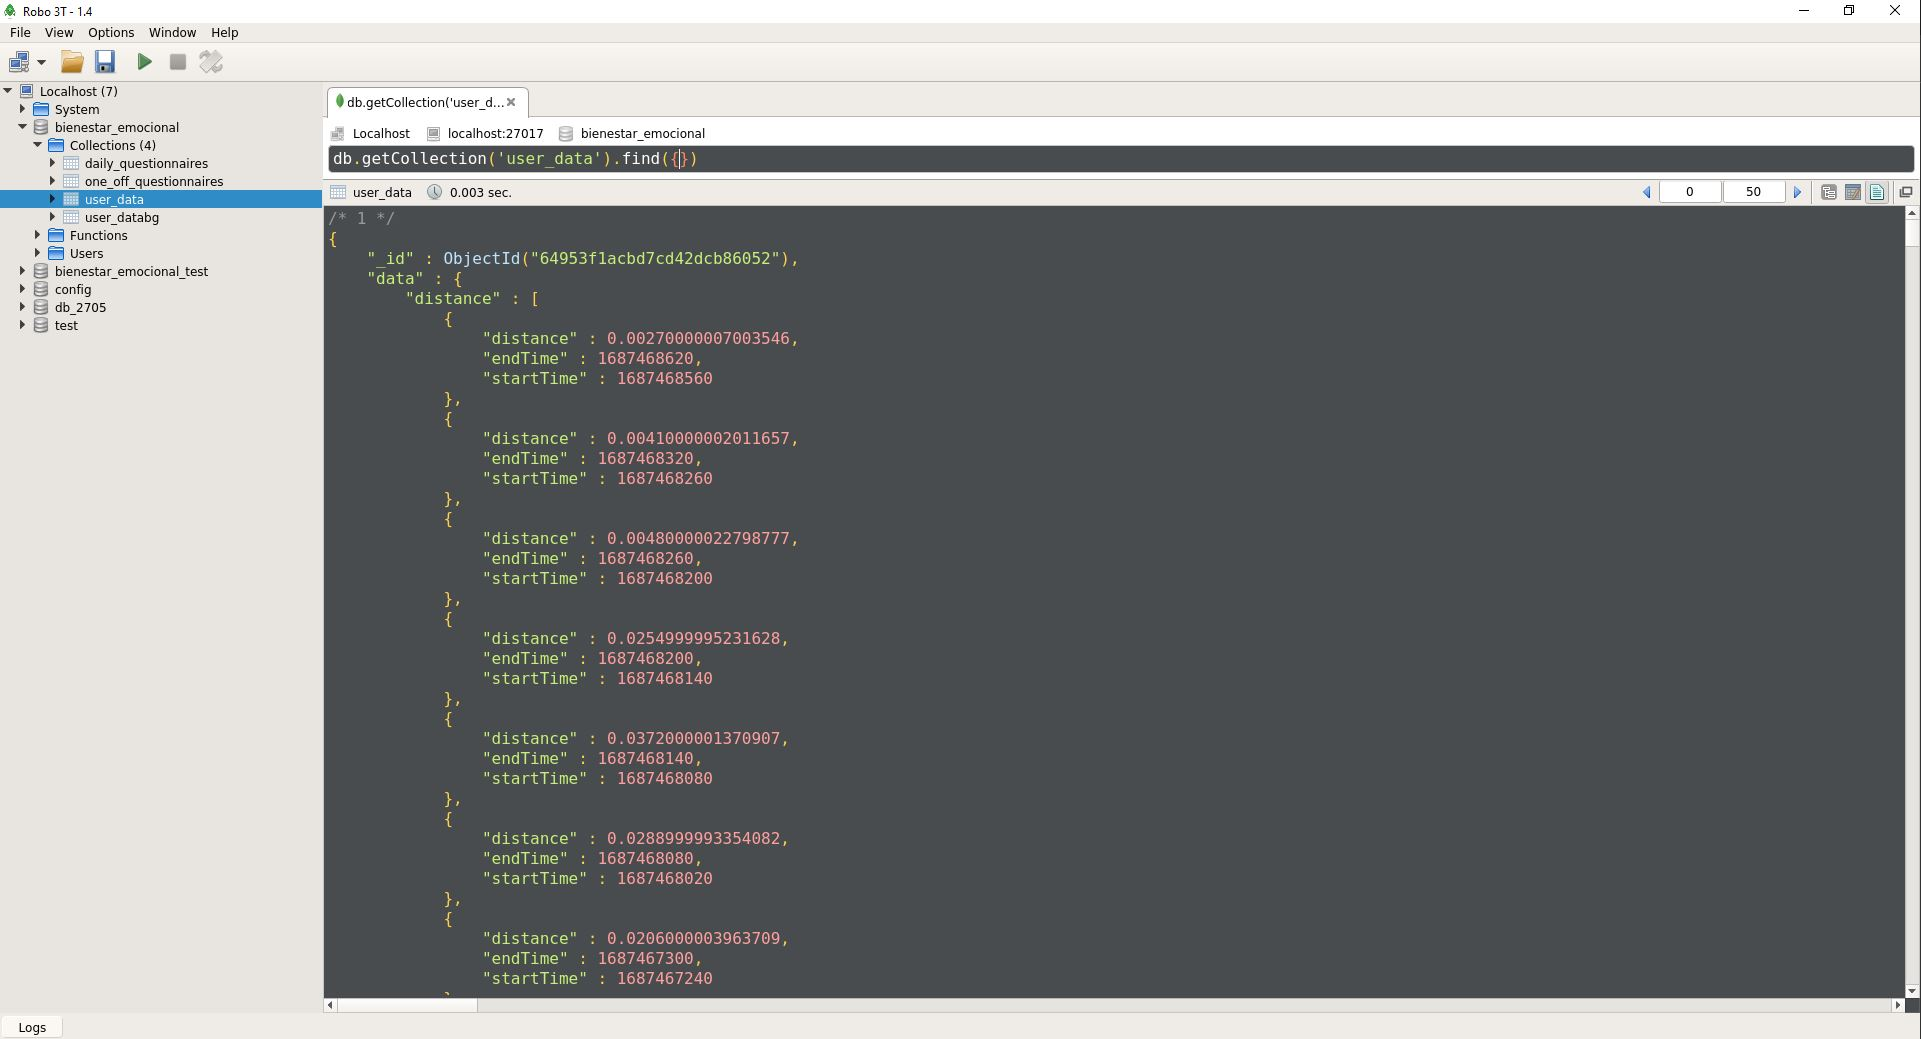
\includegraphics[width=1\textwidth]{figures/pruebas/robo3t_actividad_fisica.JPG}
                \caption{Evidencia de la \textit{Visualización general de los datos de actividad física}}
                \label{figure:pruebas:visualizacion_general_actividad}
            \end{figure}
        
        \subsection*{Caso de prueba \textit{Visualización general de los datos de seguimiento}}

            Análogamente al caso anterior, se realiza la conexión a las colecciones \textit{daily questionnaires} y \textit{one off questionnaires} mediante \textit{robo3t}, recogiéndose las respectivas evidencias en las Figuras \ref{figure:pruebas:visualizacion_general_daily} y \ref{figure:pruebas:visualizacion_general_one_off}.

            \begin{figure}[h]
                \centering
                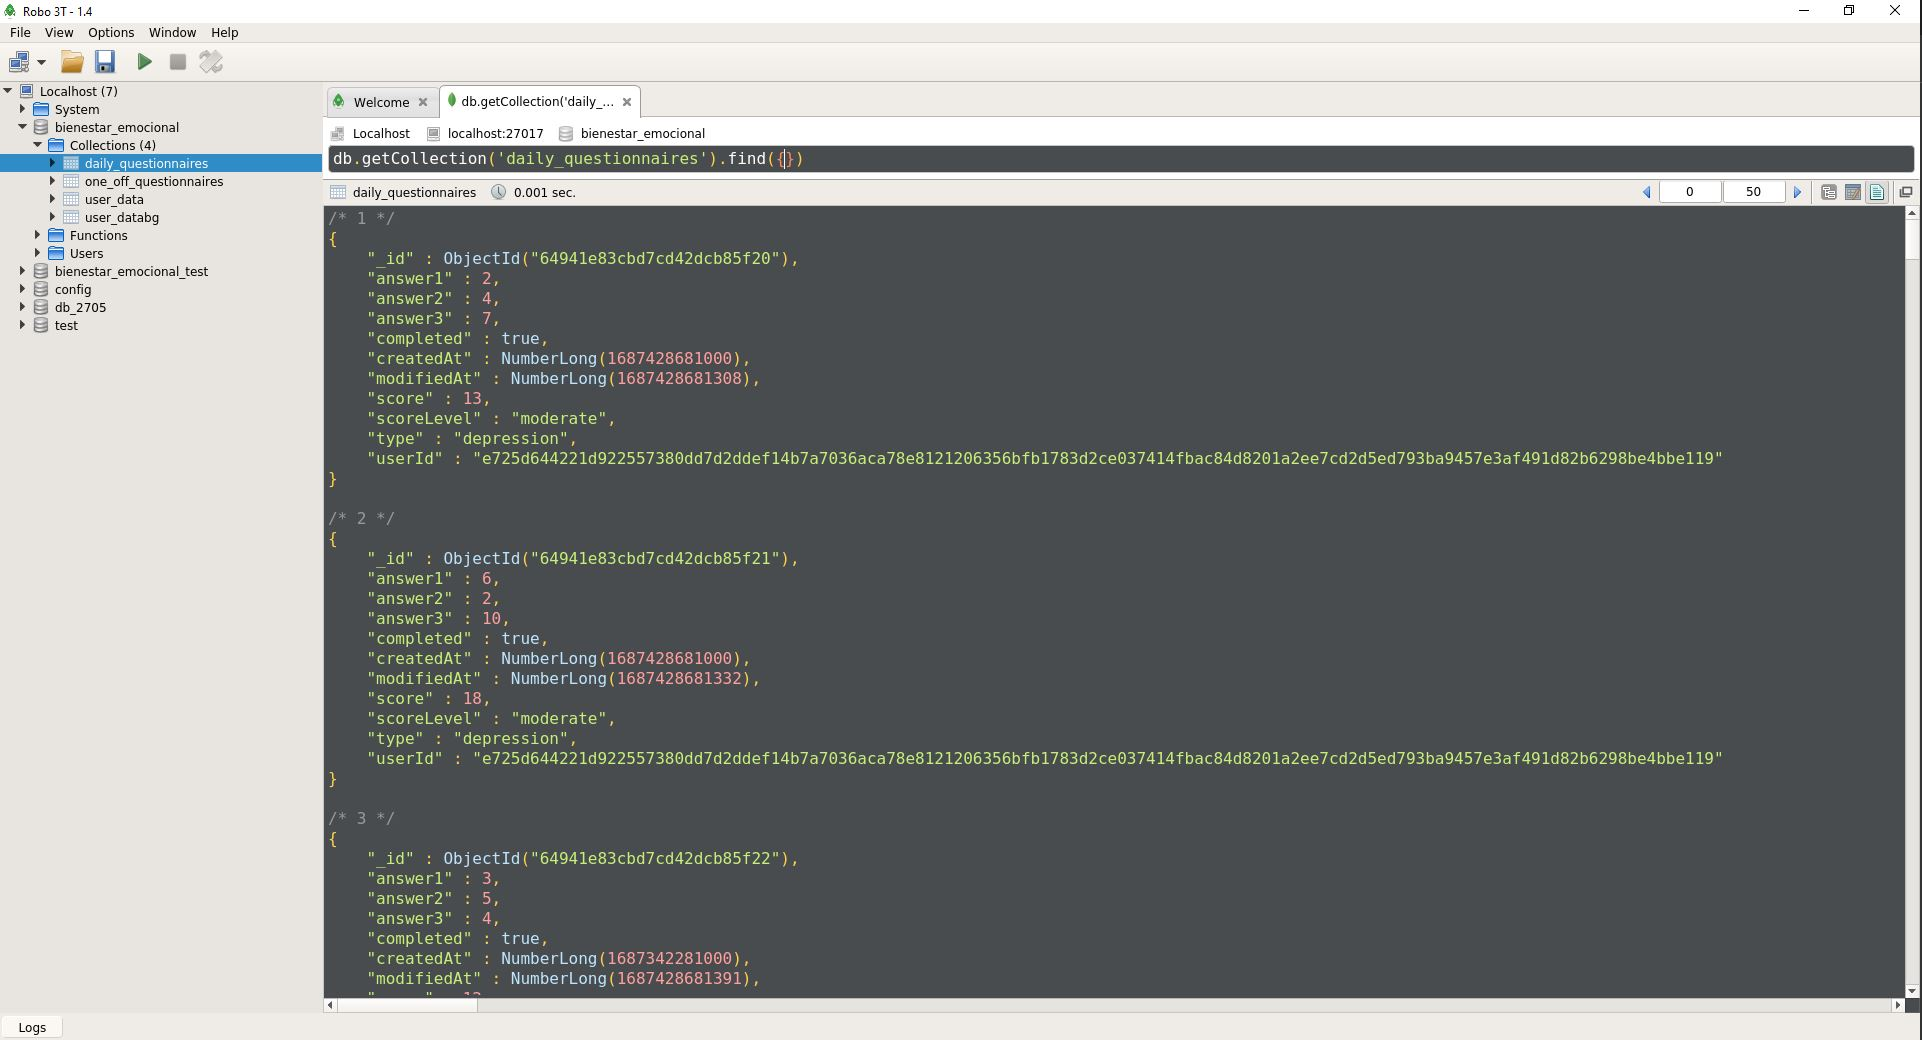
\includegraphics[width=1\textwidth]{figures/pruebas/robo3t_daily.JPG}
                \caption{Evidencia del acceso a la colección \textit{daily questionnaires}}
                \label{figure:pruebas:visualizacion_general_daily}
            \end{figure}

            \begin{figure}[h]
                \centering
                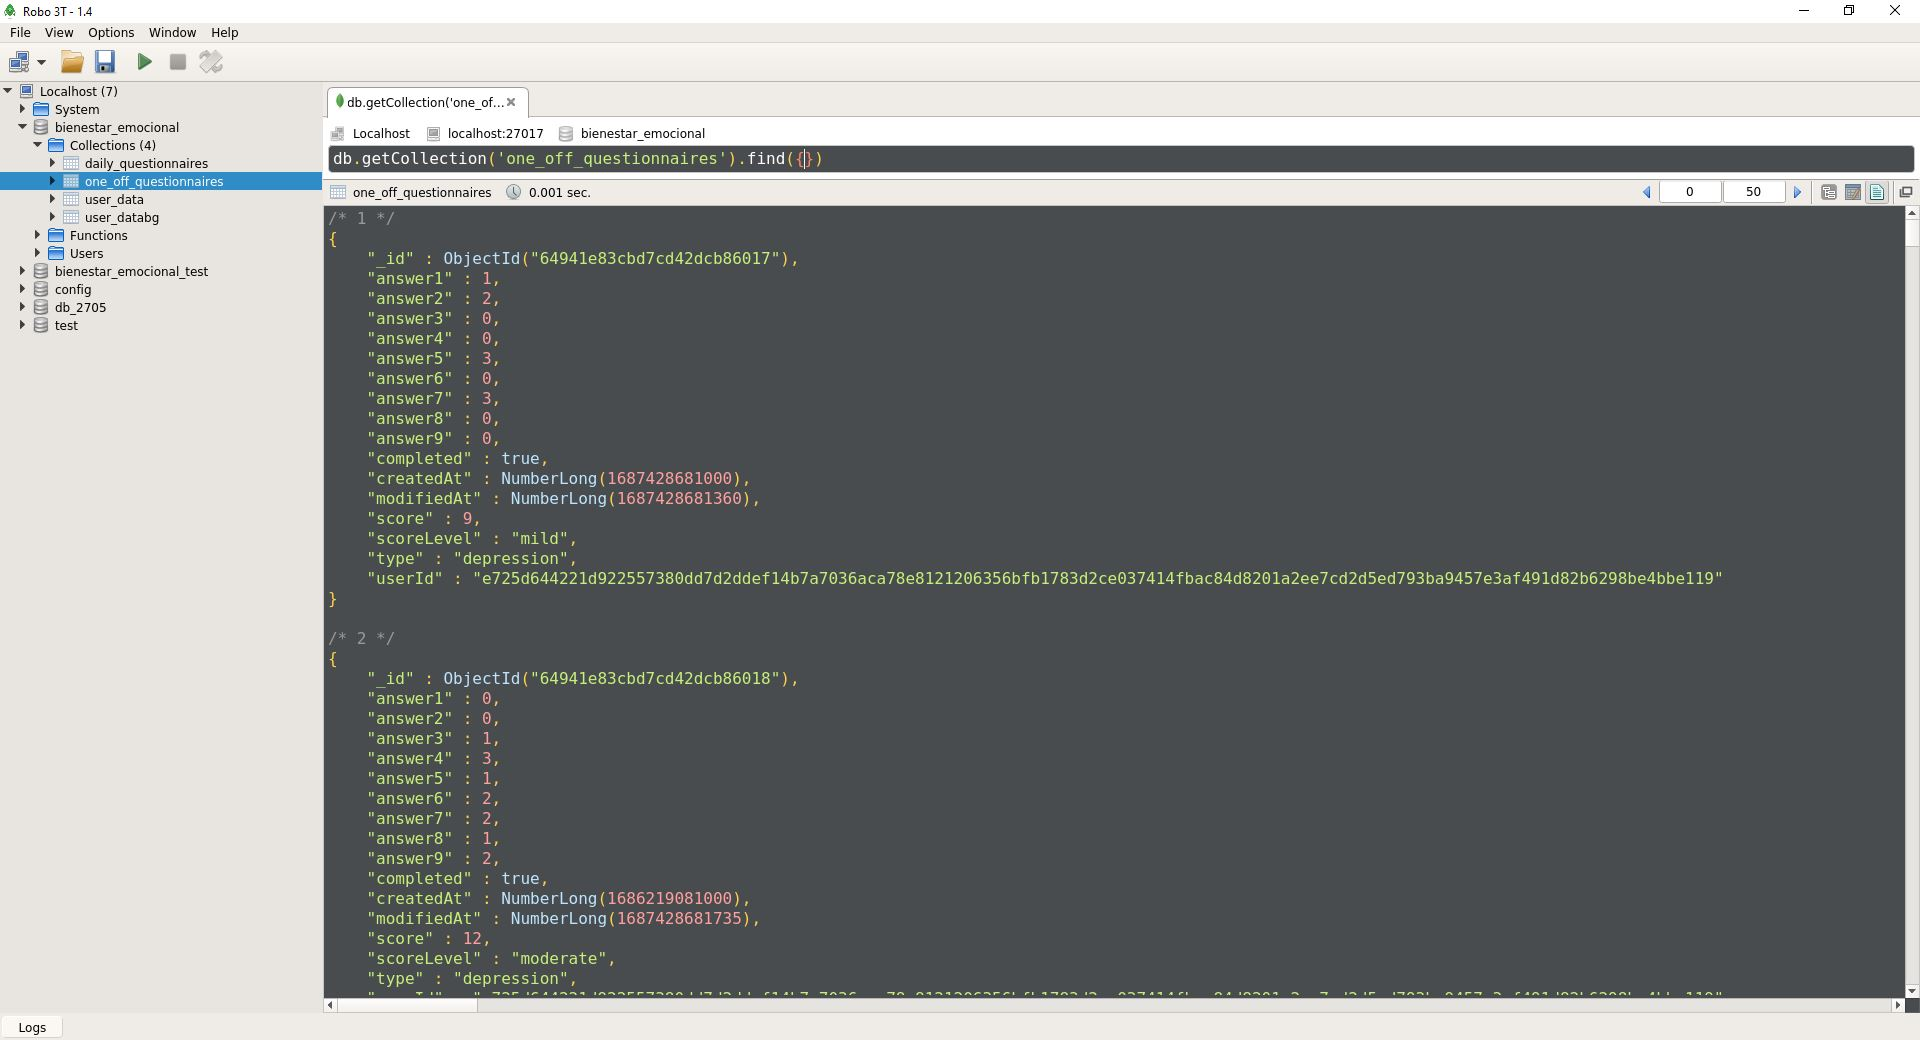
\includegraphics[width=1\textwidth]{figures/pruebas/robo3t_one_off.JPG}
                \caption{Evidencia del acceso a la colección \textit{one off questionnaires}}
                \label{figure:pruebas:visualizacion_general_one_off}
            \end{figure}

            \clearpage  % Asegura que todas las figuras y tablas pendientes se impriman antes de continuar.
    
    \section{Pruebas unitarias del componente aplicación}
    
        En esta sección se van a describir las pruebas realizadas a las funcionalidades que residen en exclusiva en el componente aplicación.

        \subsection*{Caso de prueba \textit{Primer uso de la aplicación}} 
            En este caso de prueba se pretende visualizar lo presentado al usuario cuando abre la aplicación por primera vez según lo especificado en la descripción extendida del caso de uso, recogida en la Tabla \ref{tabla:casos_uso:primer_uso}.

            Las Figuras \ref{figure:pruebas:primer_uso_bienvenida}, \ref{figure:pruebas:primer_uso_permisos} y \ref{figure:pruebas:primer_uso_permisos_dialogos} hacen referencia a la presentación del carrousel de bienvenida, la pantalla de permisos y los diálogos de aceptación de permisos, respectivamente.

            \begin{figure}[h]
                \centering
                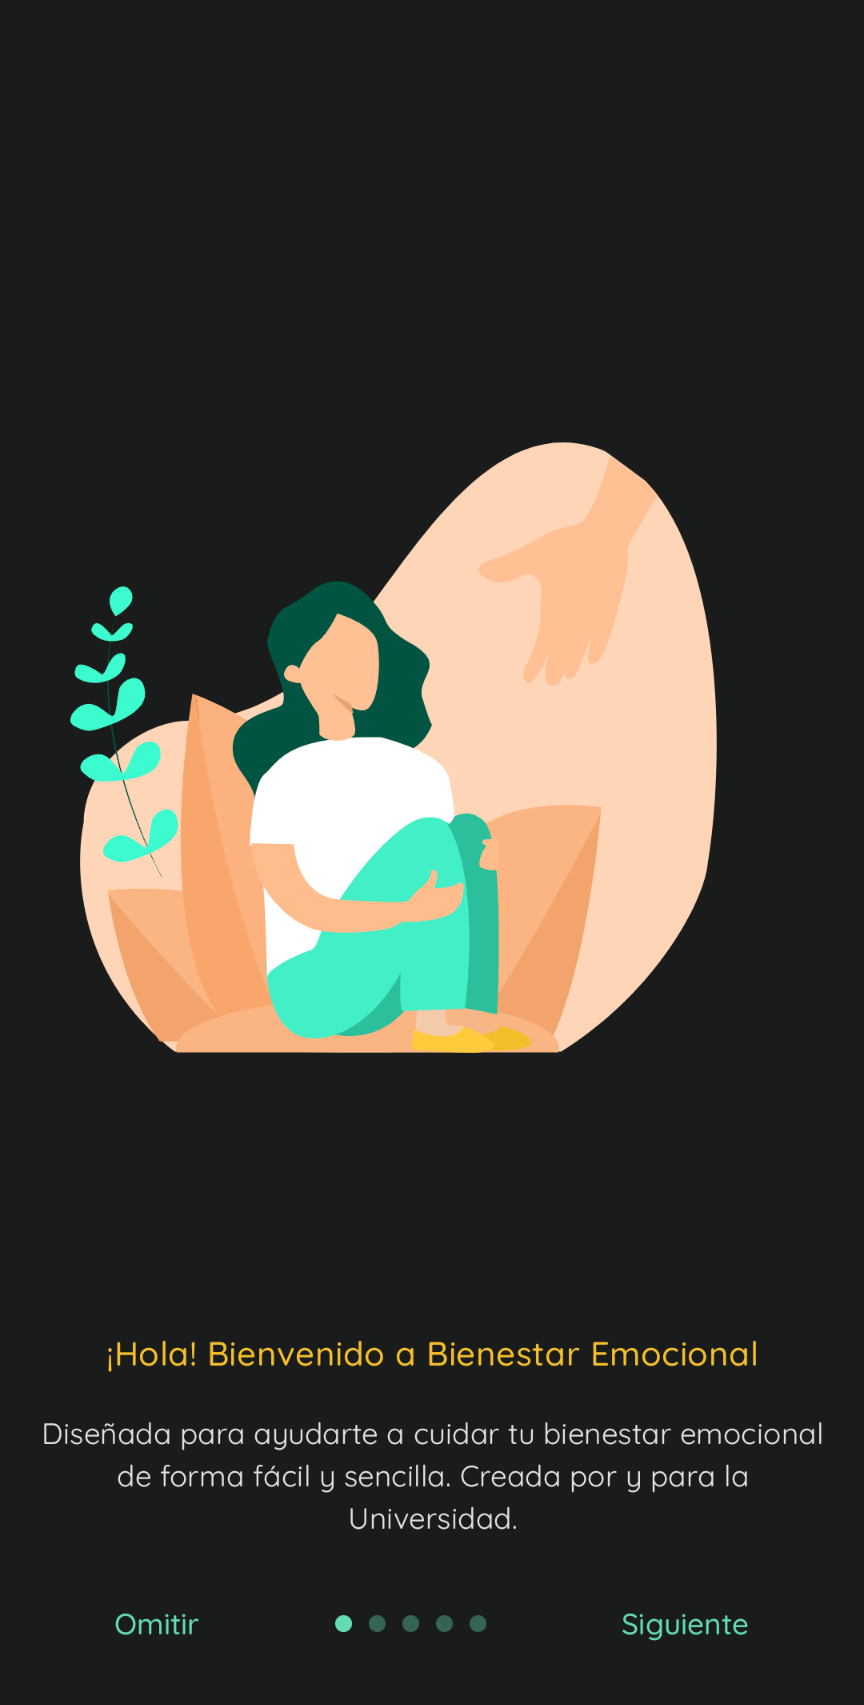
\includegraphics[width=0.32\textwidth]{figures/pruebas/primer_uso/Onboarding 1.png}
                \caption{Primer uso de la aplicación: bienvenida}
                \label{figure:pruebas:primer_uso_bienvenida}
            \end{figure}

            \begin{figure}[h]
                \centering
                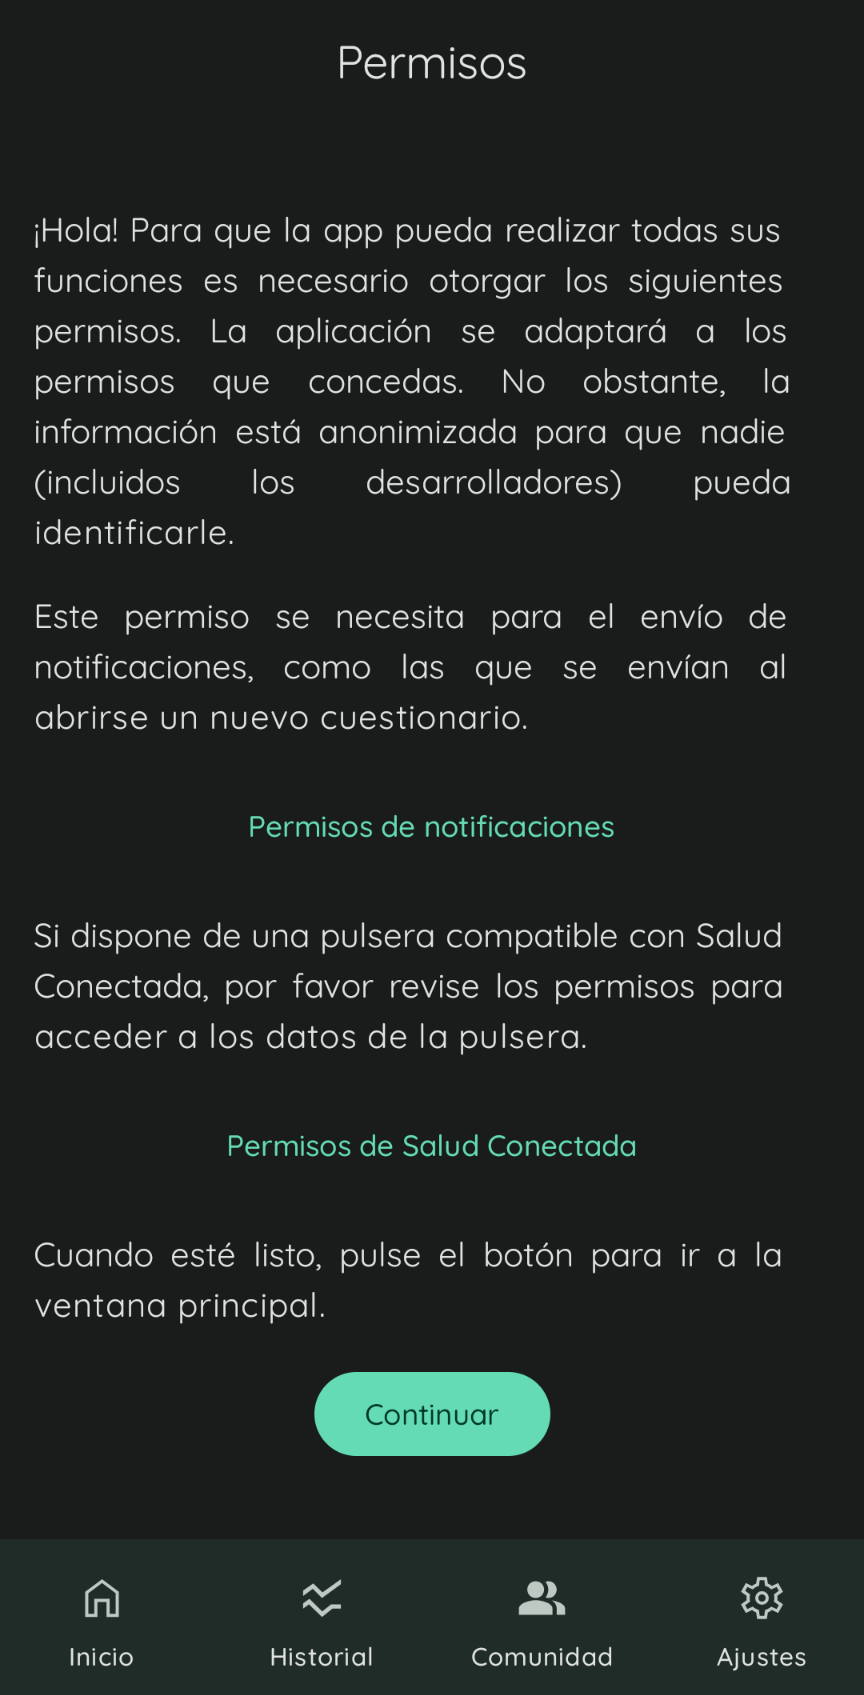
\includegraphics[width=0.32\textwidth]{figures/pruebas/primer_uso/Permisos.png}
                \caption{Primer uso de la aplicación: permisos}
                \label{figure:pruebas:primer_uso_permisos}
            \end{figure}
            
            \begin{figure}[htbp]
                \centering
                \begin{subfigure}[c]{0.32\textwidth}
                    \centering
                    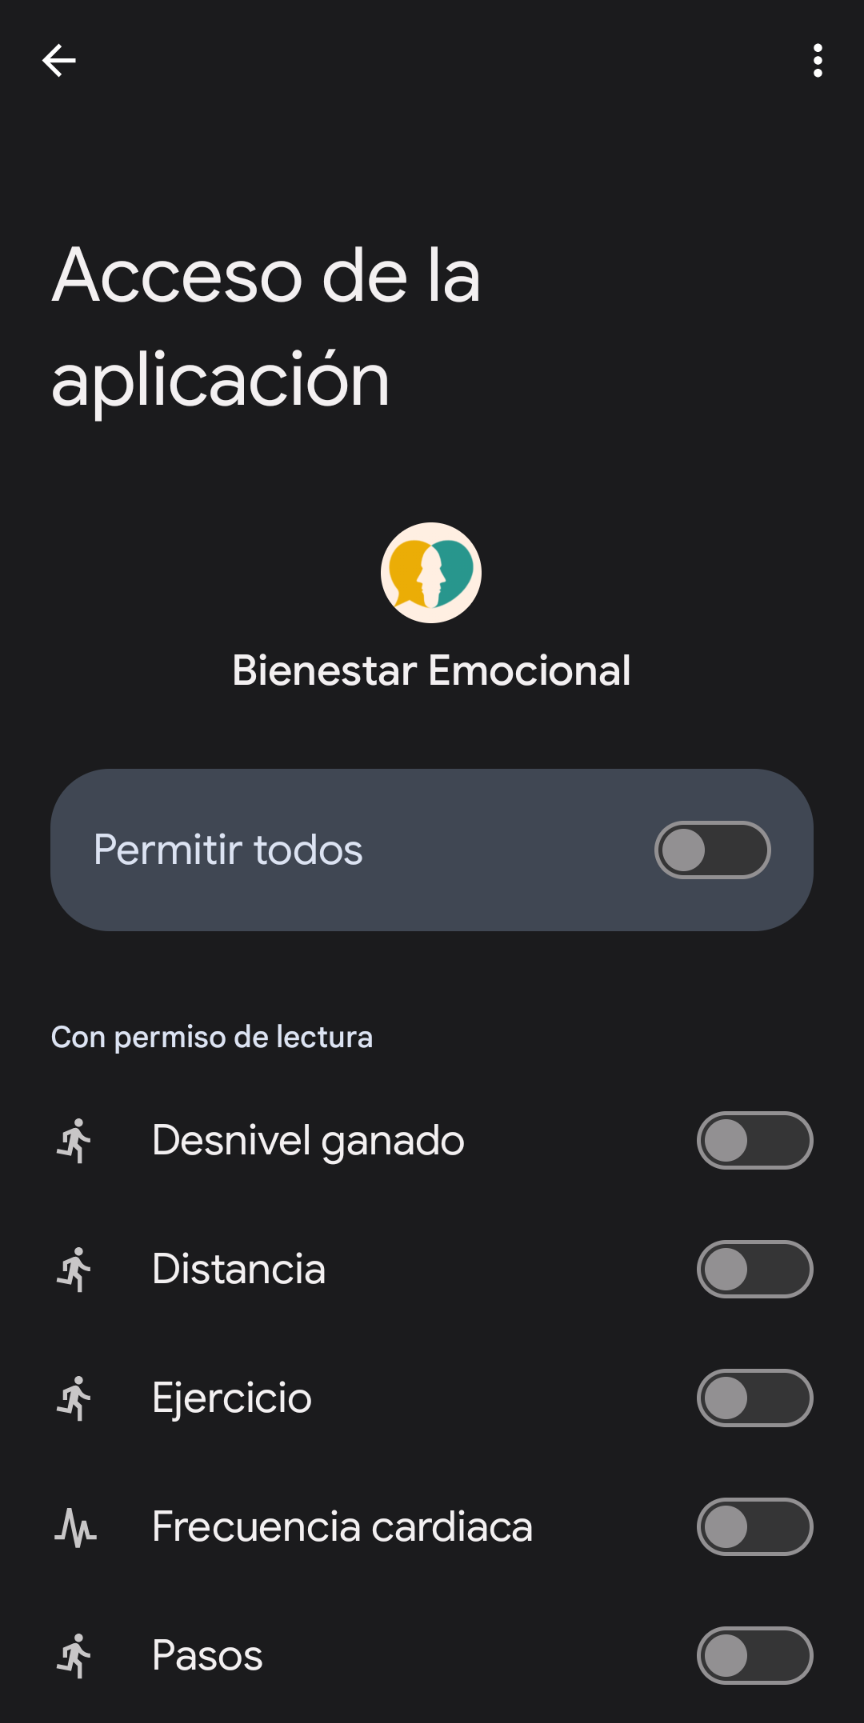
\includegraphics[width=1\textwidth]{figures/pruebas/primer_uso/Permisos HC.png}
                \end{subfigure}
                \hspace{0.1\textwidth}
                \begin{subfigure}[c]{0.32\textwidth}
                    \centering
                    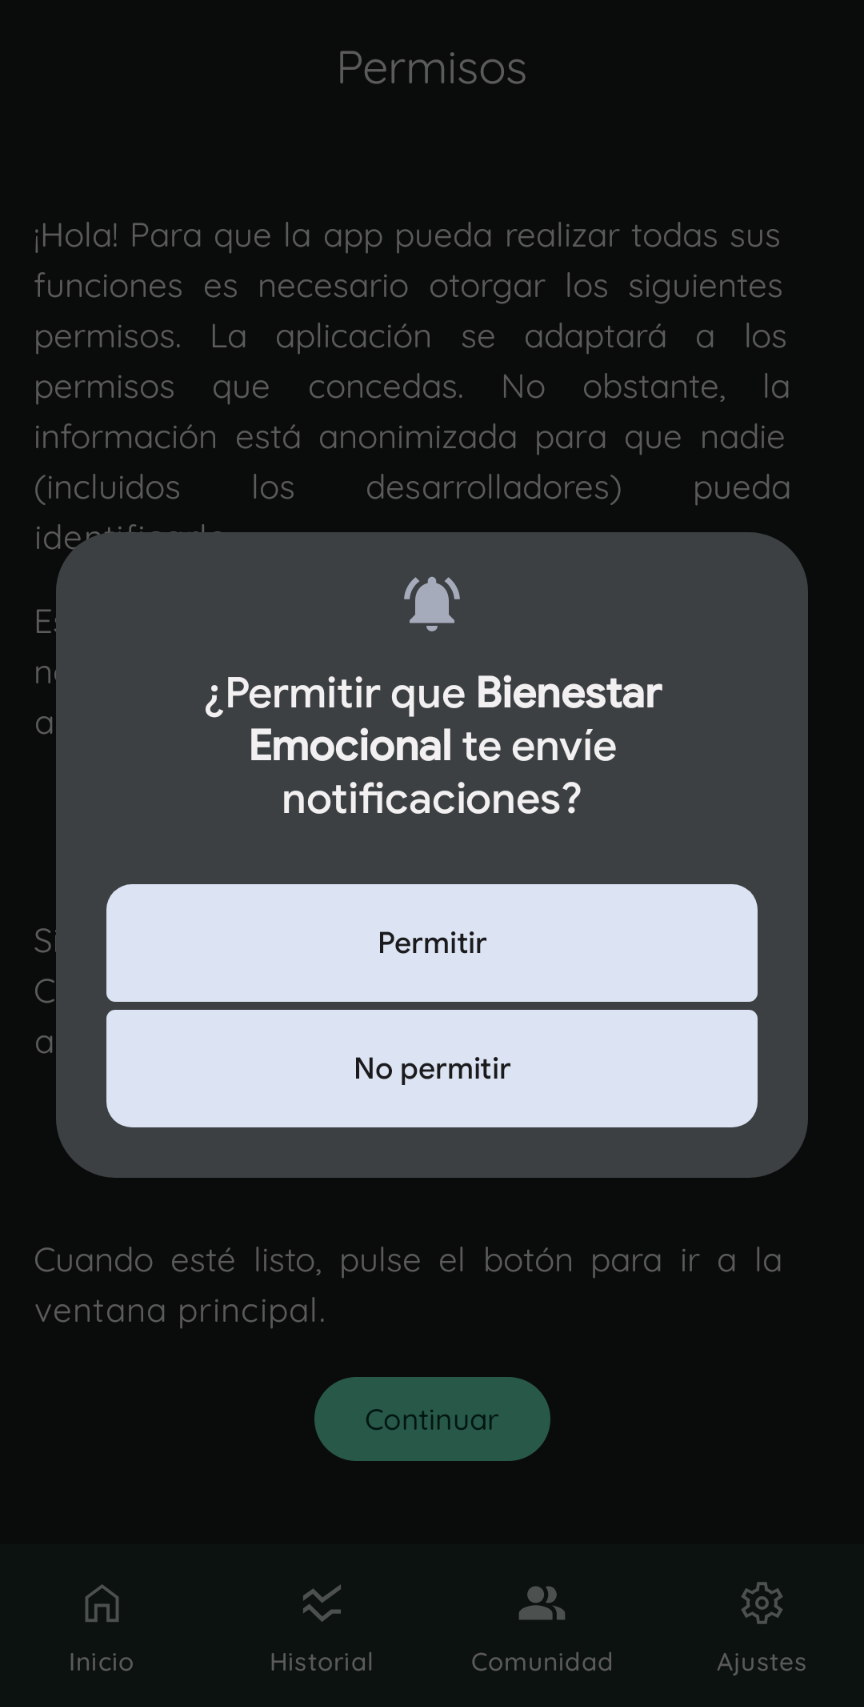
\includegraphics[width=1\linewidth]{figures/pruebas/primer_uso/Notificaciones.png}
                \end{subfigure}
                \caption{Primer uso de la aplicación: diálogos de permisos}
                \label{figure:pruebas:primer_uso_permisos_dialogos}
            \end{figure}

        \clearpage  % Asegura que todas las figuras y tablas pendientes se impriman antes de continuar.
            
        \subsection*{Caso de prueba \textit{Visualización local de los datos del wearable}}

            En esta ocasión se desea contemplar el proceso de visualización de los datos del \gls{wearable}. La Figura \ref{figure:pruebas:visualizacion_local:habitual} muestra al flujo habitual, mientras la Figura \ref{figure:pruebas:visualizacion_local:alternativo} muestra el flujo de falta de permisos. 

            \begin{figure}[htbp]
                \centering
                \begin{subfigure}[c]{0.27\textwidth}
                    \centering
                    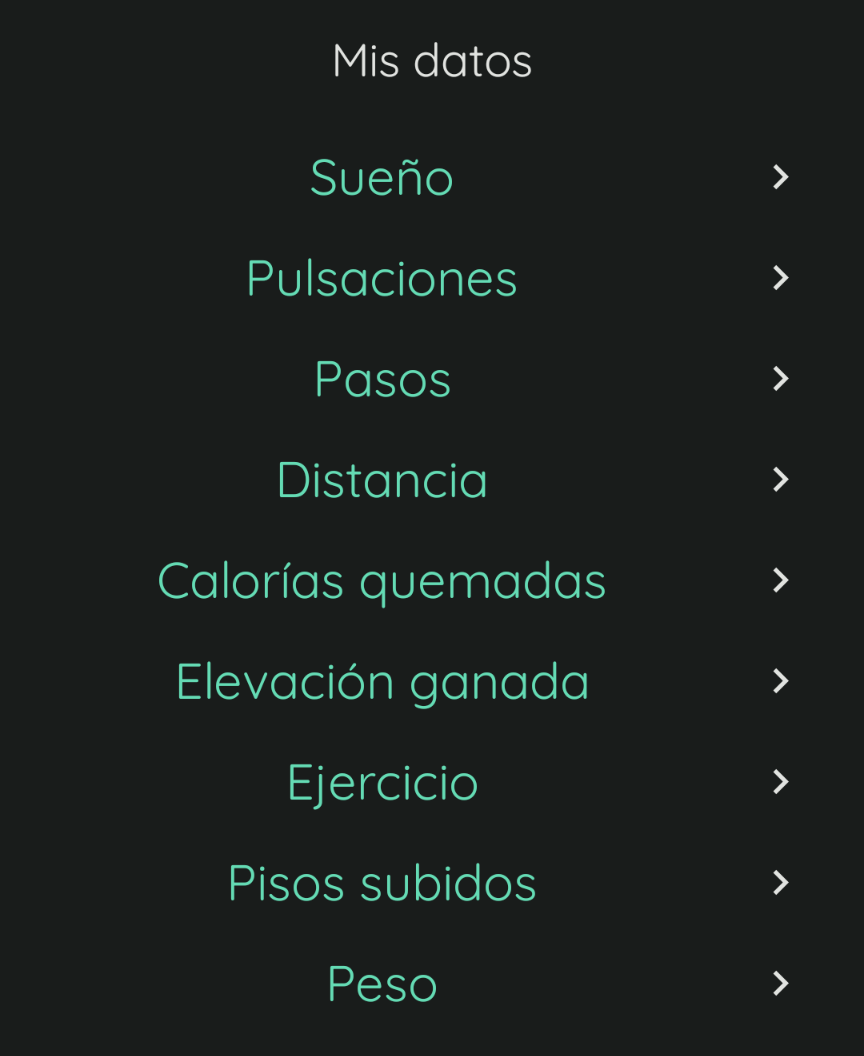
\includegraphics[width=1\textwidth]{figures/pruebas/local_wearable/Listado general.png}
                \end{subfigure}
                \hspace{0.1\textwidth}
                \begin{subfigure}[c]{0.27\textwidth}
                    \centering
                    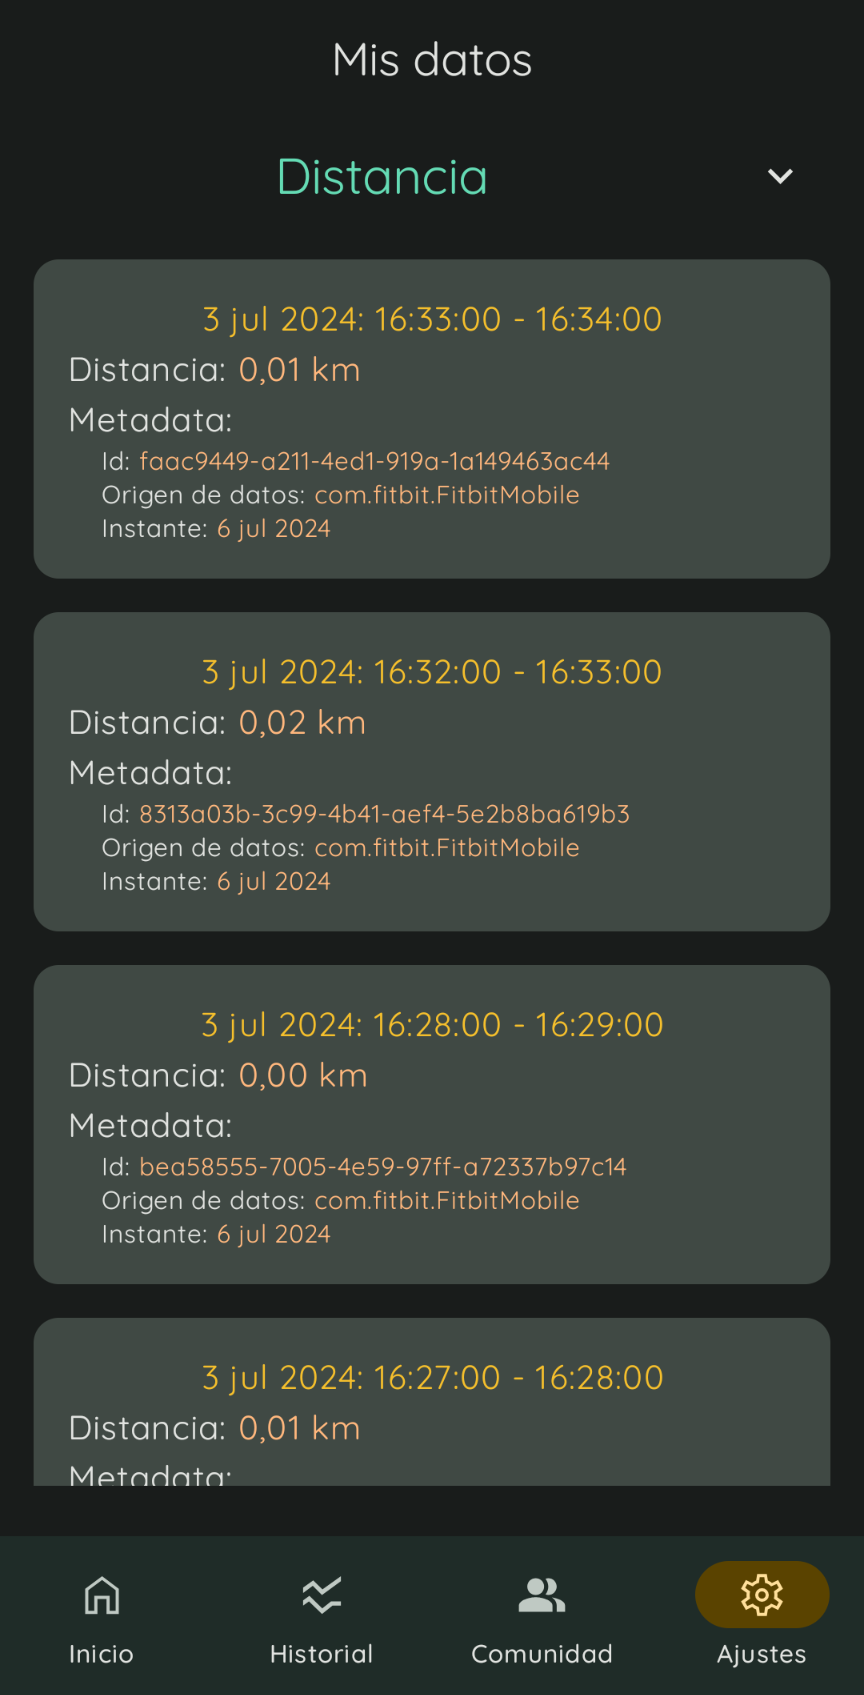
\includegraphics[width=1\linewidth]{figures/pruebas/local_wearable/Datos distancia.png}
                \end{subfigure}
                \caption{Visualización local de los datos del wearable: flujo habitual}
                \label{figure:pruebas:visualizacion_local:habitual}
            \end{figure}

            \begin{figure}[htbp]
                \centering
                \begin{subfigure}[c]{0.27\textwidth}
                    \centering
                    
\includegraphics[width=1\textwidth]{figures/pruebas/local_wearable/Distancia sin permiso.png}
                \end{subfigure}
                \hspace{0.1\textwidth}
                \begin{subfigure}[c]{0.27\textwidth}
                    \centering
                    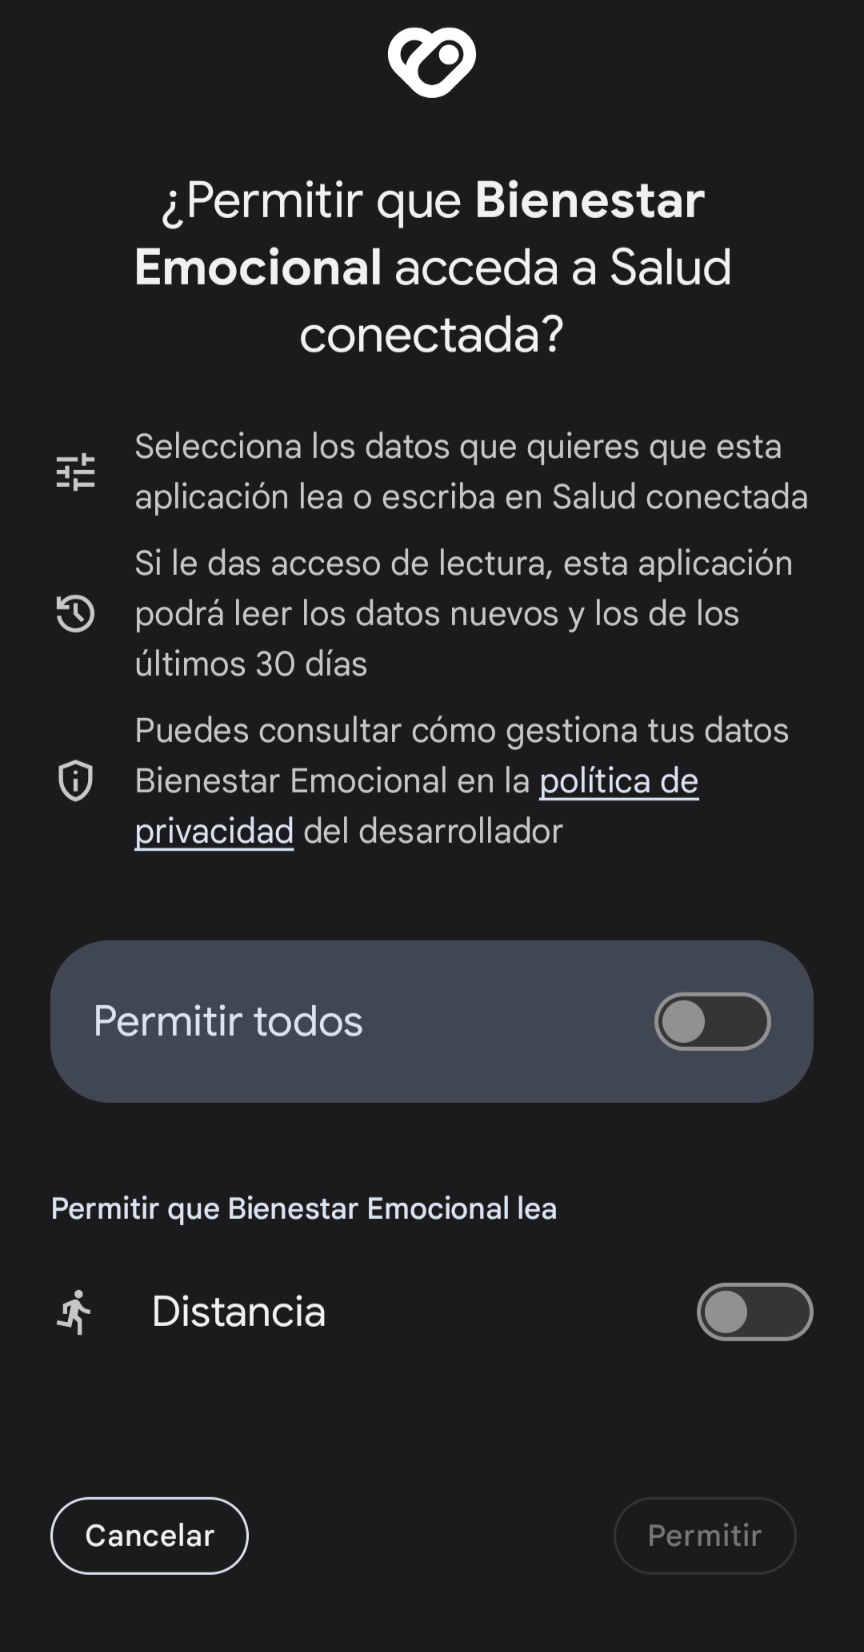
\includegraphics[width=1\linewidth]{figures/pruebas/local_wearable/Permiso distancia.png}
                \end{subfigure}
                \caption{Visualización local de los datos del wearable: flujo alternativo}
                \label{figure:pruebas:visualizacion_local:alternativo}
            \end{figure}

            \clearpage  % Asegura que todas las figuras y tablas pendientes se impriman antes de continuar.
            
        \subsection*{Caso de prueba \textit{Recepción de notificaciones}} 
            Las Figuras \ref{figure:pruebas:notificacion_manana}, \ref{figure:pruebas:notificacion_noche} y \ref{figure:pruebas:notificacion_puntual} muestran las notificaciones en el dispositivo del autor relativas a las rondas de cuestionarios disponibles en la aplicación.
            
            \begin{figure}[h]
                \centering
                
\includegraphics[width=0.4\textwidth]{figures/pruebas/notificaciones/Notificacion manana.png}
                \caption{Evidencia de la notificación de cuestionarios de mañana}
                \label{figure:pruebas:notificacion_manana}
            \end{figure}

            \begin{figure}[h]
                \centering
                
\includegraphics[width=0.4\textwidth]{figures/pruebas/notificaciones/Notificacion noche.png}
                \caption{Evidencia de la notificación de cuestionarios de noche}
                \label{figure:pruebas:notificacion_noche}
            \end{figure}
            
            \begin{figure}[h]
                \centering
                
\includegraphics[width=0.4\textwidth]{figures/pruebas/notificaciones/Notificacion puntual.png}
                \caption{Evidencia de la notificación de cuestionarios puntuales}
                \label{figure:pruebas:notificacion_puntual}
            \end{figure}

        \subsection*{Caso de prueba \textit{Realización y guardado de cuestionario}} 
            En este caso de prueba se desea visualizar cómo son los cuestionarios mostrados al usuario y el guardado de los mismos en base de datos. En este caso, los ejemplos planteados son en base a un cuestionario de depresión puntual.

            En primer lugar, la aplicación muestra al usuario el cuestionario, como refleja la Figura \ref{figure:pruebas:realizacion_cuestionario:presentacion}.

            \begin{figure}[h]
                \centering
                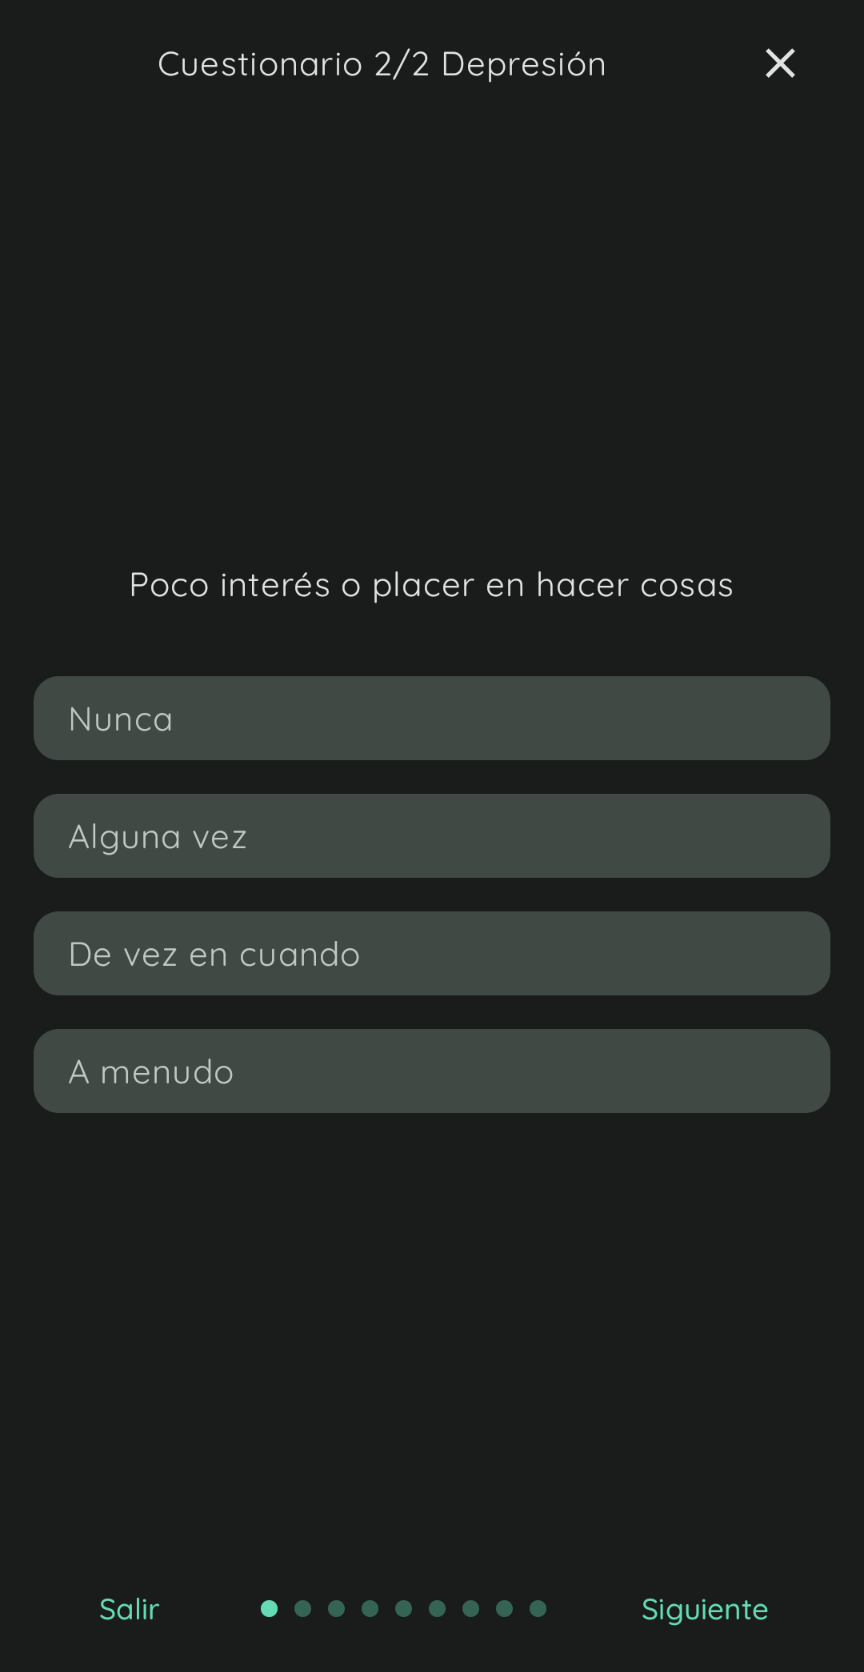
\includegraphics[width=0.4\textwidth]{figures/pruebas/realizacion_cuestionario/Presentacion.png}
                \caption{Realización y guardado de cuestionario: presentación}
                \label{figure:pruebas:realizacion_cuestionario:presentacion}
            \end{figure}

            Cuando el cuestionario termina la aplicación guarda en base de datos los resultados. La Figura \ref{figure:pruebas:realizacion_cuestionario:guardado}, muestra el almacenamiento de esos datos a través del \textit{App Inspector} de \textit{Android Studio}.

            \begin{figure}[h]
                \centering
                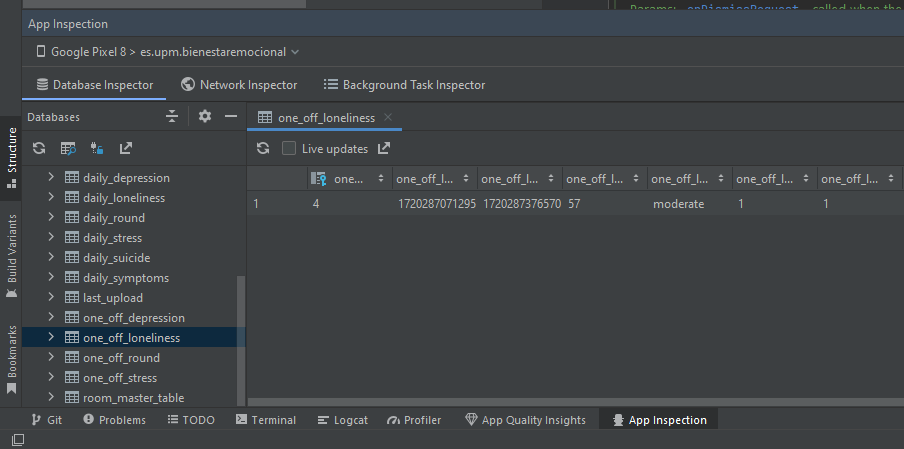
\includegraphics[width=1\textwidth]{figures/pruebas/realizacion_cuestionario/Guardado.png}
                \caption{Realización y guardado de cuestionario: guardado}
                \label{figure:pruebas:realizacion_cuestionario:guardado}
            \end{figure}

            En el caso de que queden preguntas por responder o si el usuario desea omitir el cuestionario se muestran los diálogos reflejados en la Figura \ref{figure:pruebas:visualizacion_local:dialogos}.

            \begin{figure}[htbp]
                \centering
                \begin{subfigure}[c]{0.4\textwidth}
                    \centering
                    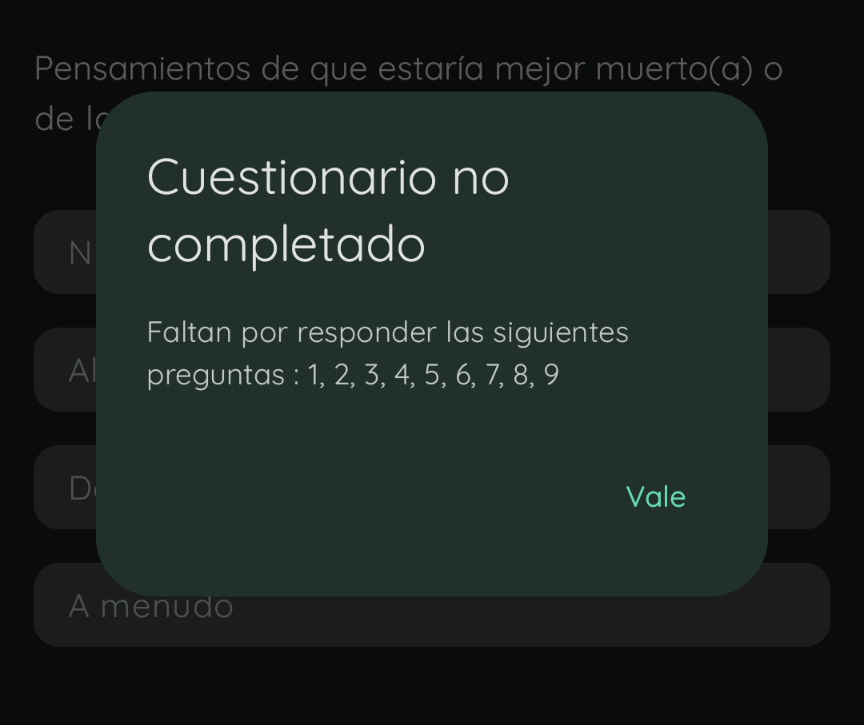
\includegraphics[width=1\textwidth]{figures/pruebas/realizacion_cuestionario/Preguntas restantes.png}
                \end{subfigure}
                \hspace{0.1\textwidth}
                \begin{subfigure}[c]{0.4\textwidth}
                    \centering
                    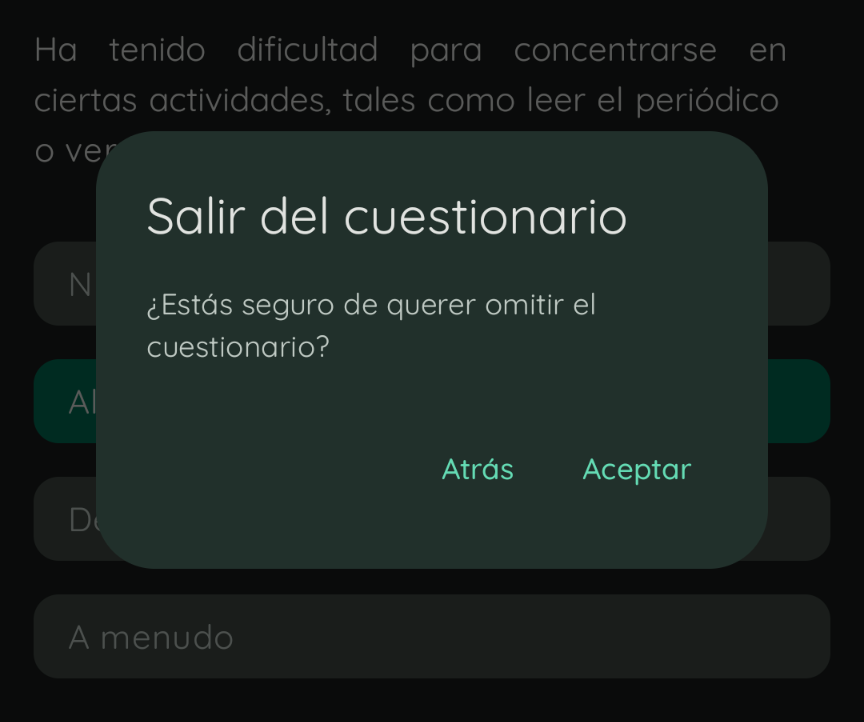
\includegraphics[width=1\linewidth]{figures/pruebas/realizacion_cuestionario/Salir del cuestionario.png}
                \end{subfigure}
                \caption{Realización y guardado de cuestionario: diálogos de aviso}
                \label{figure:pruebas:visualizacion_local:dialogos}
            \end{figure}

            \clearpage  % Asegura que todas las figuras y tablas pendientes se impriman antes de continuar.
            
        \subsection*{Caso de prueba \textit{Presentación de resultado}}
            En esta ocasión se desea demostrar cómo se presentan los resultados de los cuestionarios que tienen definidos puntuación y nivel. En la Figura \ref{figure:pruebas:presentacion_resultado:resumen} se muestra el resumen del cuestionario, mientras en la Figura \ref{figure:pruebas:presentacion_resultado:consejo} se dispone el panel del consejo ofrecido al usuario.

            \begin{figure}[h]
                \centering
                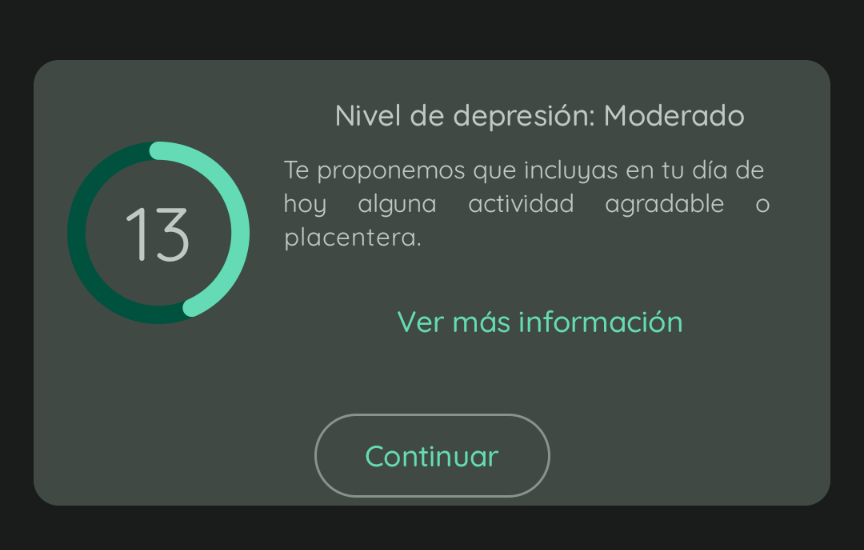
\includegraphics[width=0.4\textwidth]{figures/pruebas/presentacion_resultado/Resultado.png}
                \caption{Presentación de resultado: resumen}
                \label{figure:pruebas:presentacion_resultado:resumen}
            \end{figure}

            \begin{figure}[h]
                \centering
                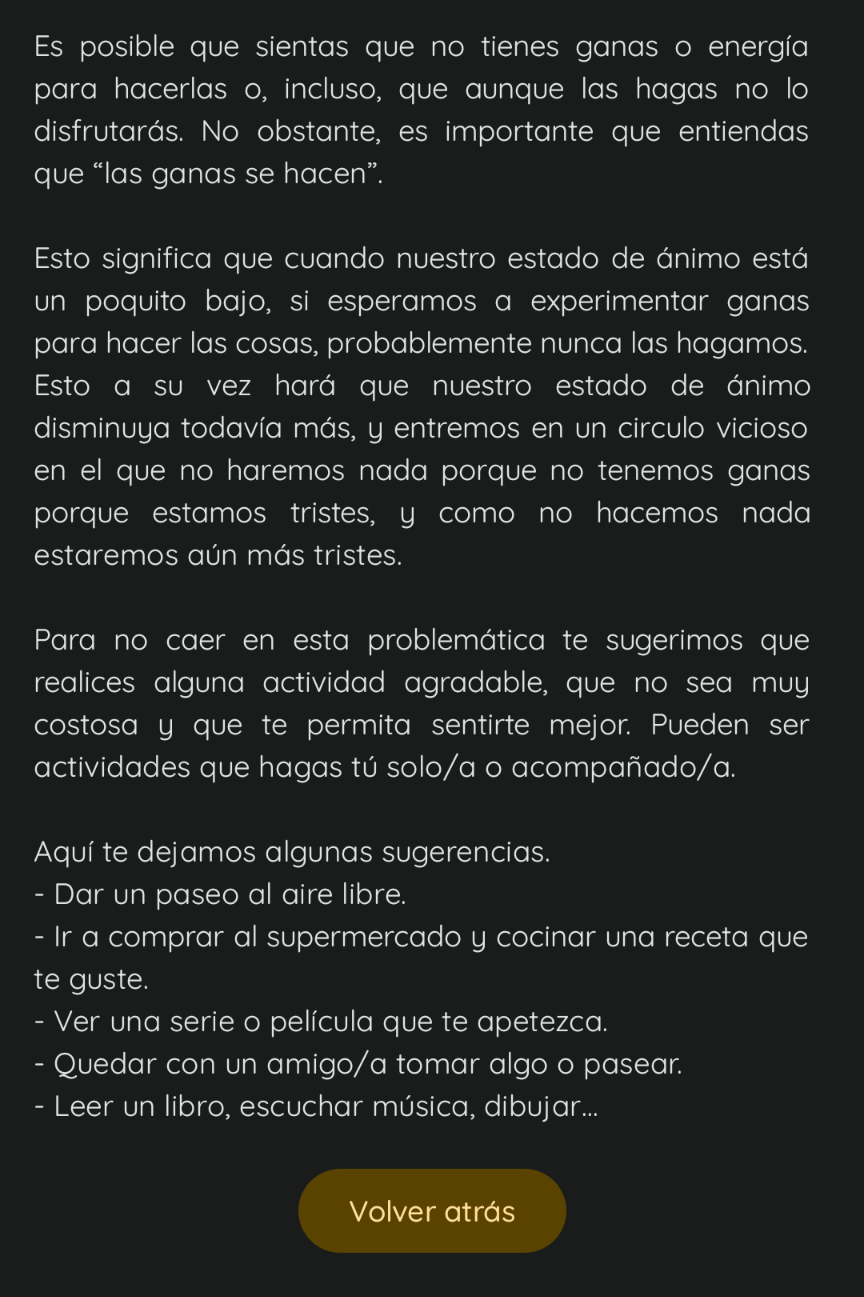
\includegraphics[width=0.4\textwidth]{figures/pruebas/presentacion_resultado/Consejo.png}
                \caption{Presentación de resultado: consejo}
                \label{figure:pruebas:presentacion_resultado:consejo}
            \end{figure}

            \clearpage  % Asegura que todas las figuras y tablas pendientes se impriman antes de continuar.
            
        \subsection*{Caso de prueba \textit{Visualización individual}}
            Esta sección muestra cómo se puede realizar la visualización individual, en este caso del estrés. La primera puede ver el usuario es el menú de inicio, mostrado en la Figura \ref{figure:pruebas:visualizacion_individual:inicio}.

            \begin{figure}[h]
                \centering
                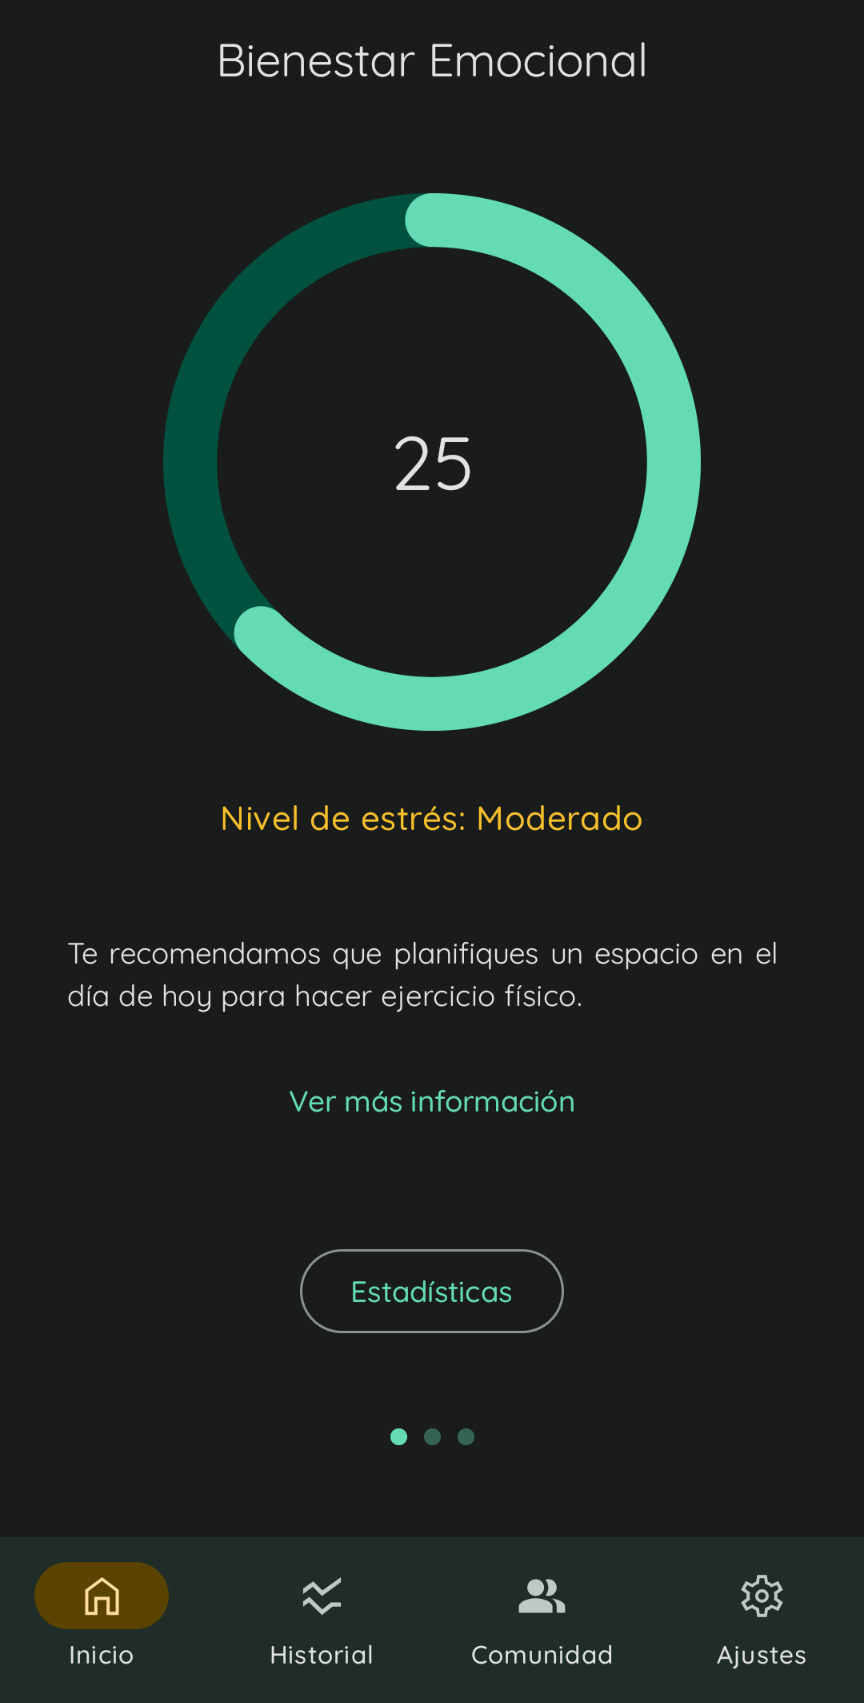
\includegraphics[width=0.4\textwidth]{figures/pruebas/visualizacion_individual/Inicio estres.png}
                \caption{Visualización individual: inicio}
                \label{figure:pruebas:visualizacion_individual:inicio}
            \end{figure}

            En este punto el usuario puede consultar el consejo asociado o los detalles de la medida en cuestión, como refleja la Figura \ref{figure:pruebas:visualizacion_individual:detalles}.

            \begin{figure}[htbp]
                \centering
                \begin{subfigure}[c]{0.4\textwidth}
                    \centering
                    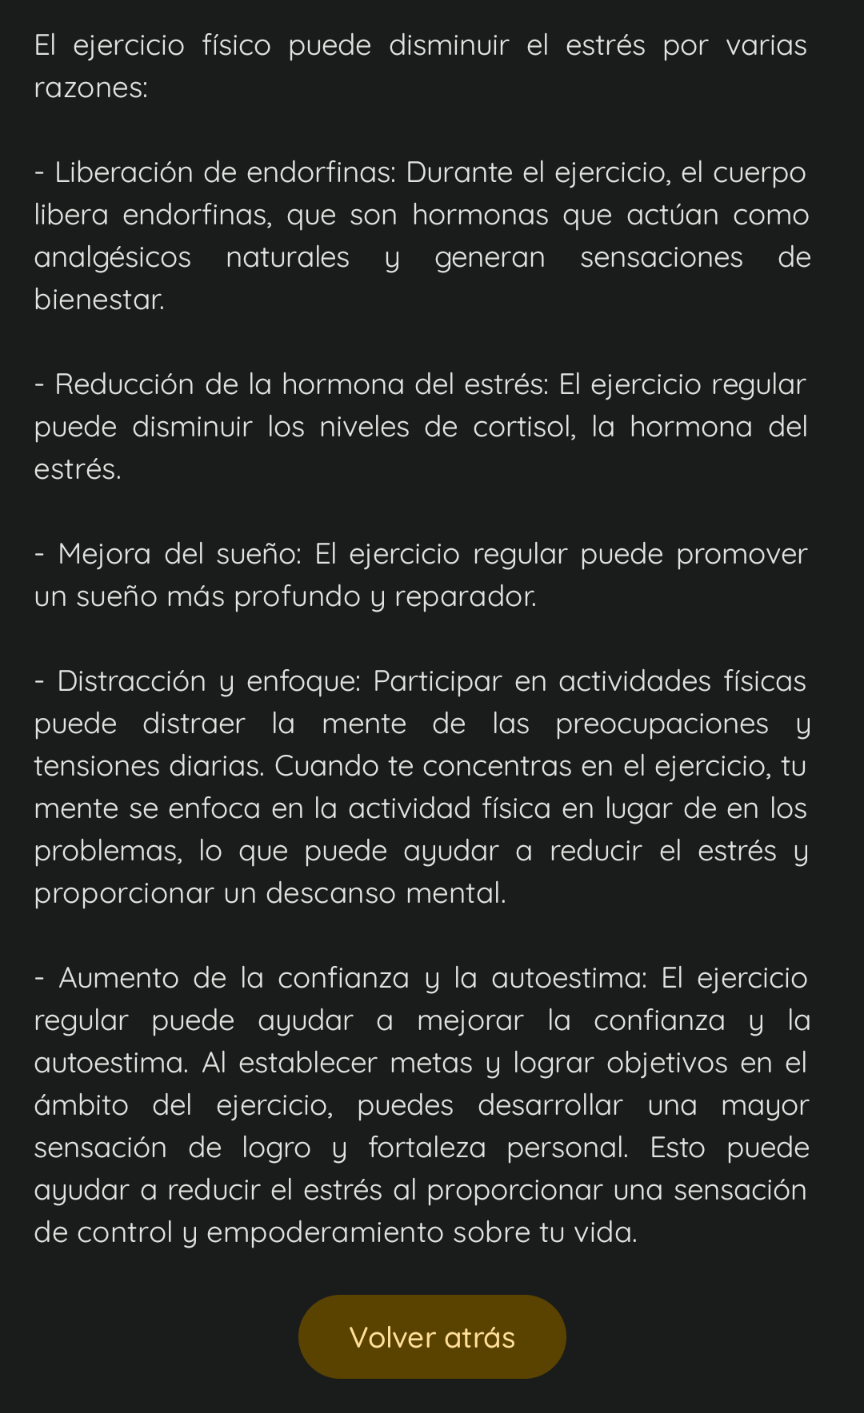
\includegraphics[width=1\textwidth]{figures/pruebas/visualizacion_individual/Consejo estres.png}
                \end{subfigure}
                \hspace{0.1\textwidth}
                \begin{subfigure}[c]{0.4\textwidth}
                    \centering
                    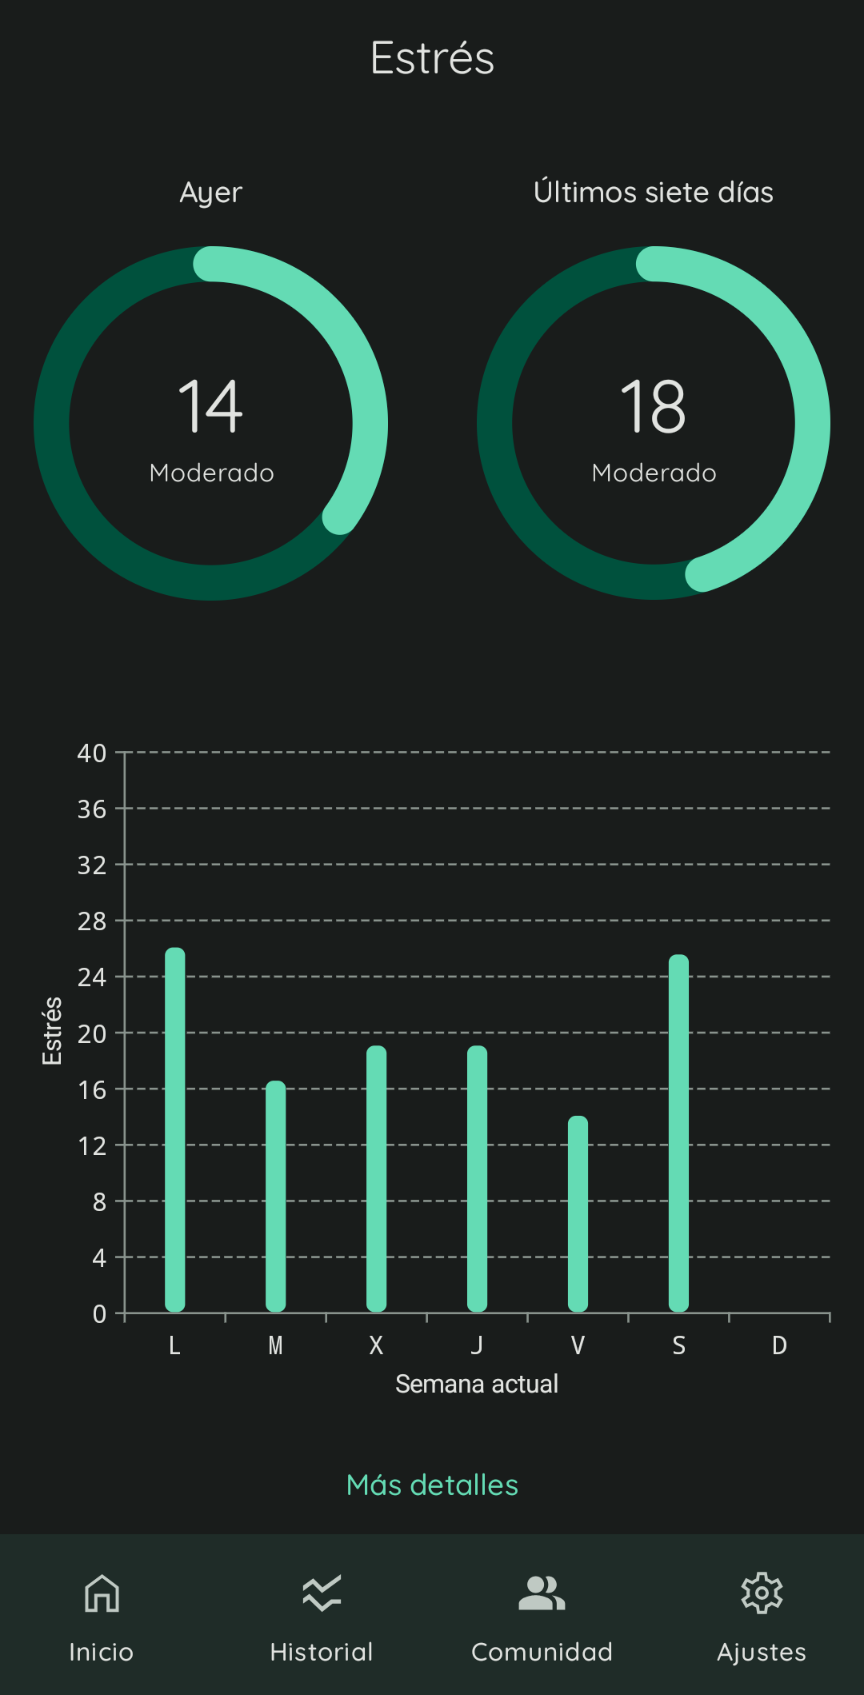
\includegraphics[width=1\linewidth]{figures/pruebas/visualizacion_individual/Medida estres.png}
                \end{subfigure}
                \caption{Visualización estadística: consejo y detalles}
                \label{figure:pruebas:visualizacion_individual:detalles}
            \end{figure}
            
            \clearpage  % Asegura que todas las figuras y tablas pendientes se impriman antes de continuar.
        \subsection*{Caso de prueba \textit{Visualización estadística}} 

            Esta sección muestra cómo se puede realizar la visualización estadística, nuevamente del estrés. El usuario puede variar entre diferentes parámetros, pero por simplificar, la Figura \ref{figure:pruebas:visualizacion_estadistica} refleja la agrupación por día y mes, respectivamente.

            \begin{figure}[htbp]
                \centering
                \begin{subfigure}[c]{0.4\textwidth}
                    \centering
                    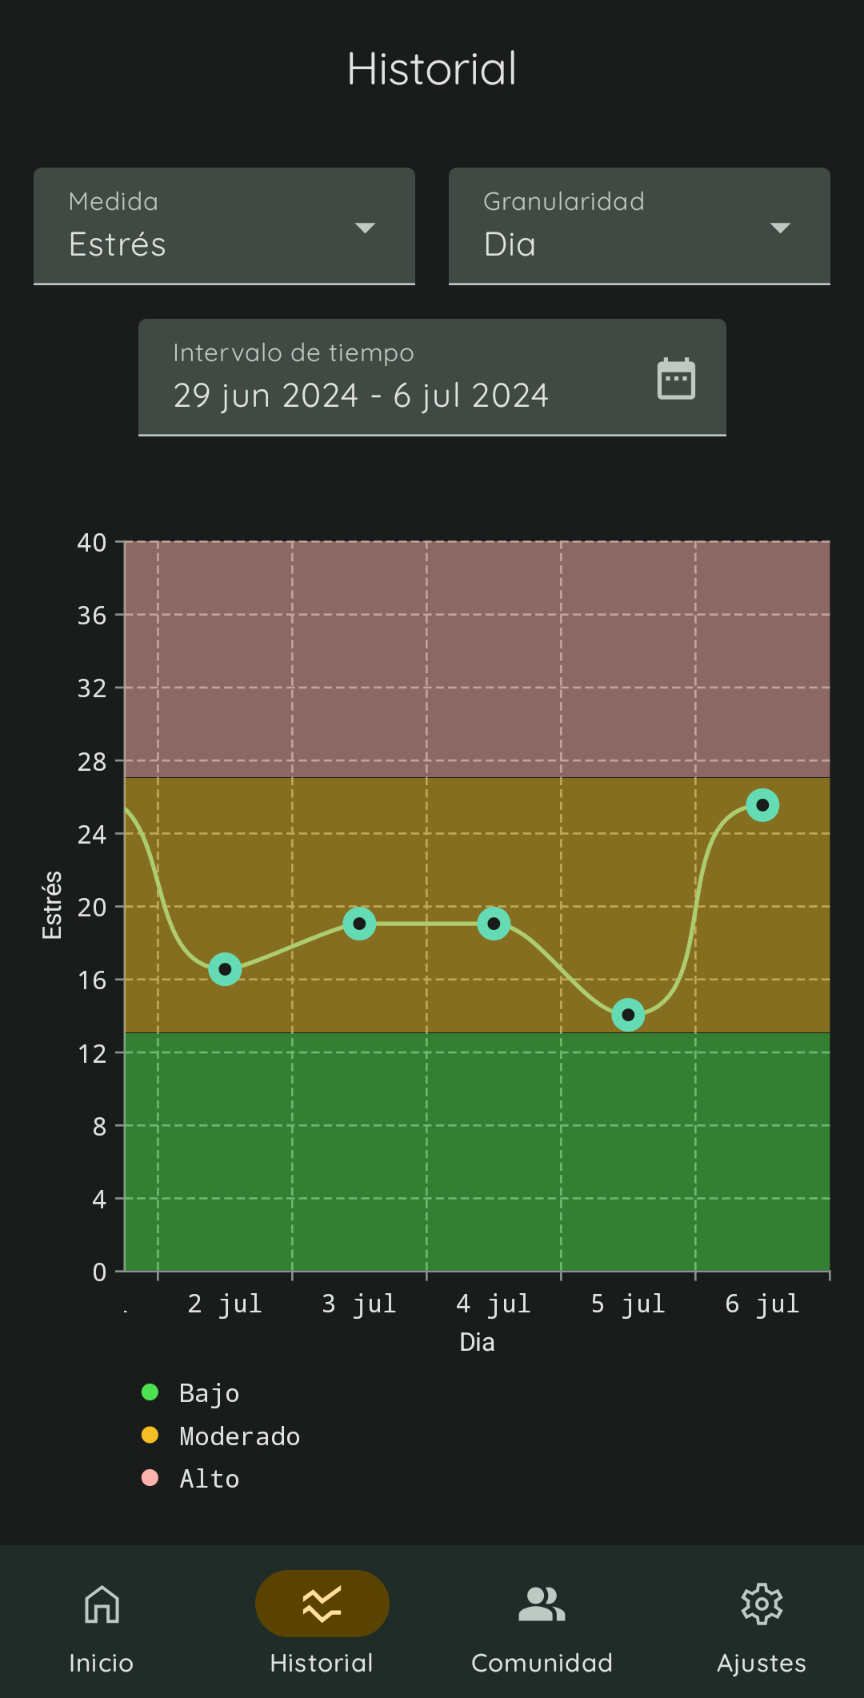
\includegraphics[width=1\textwidth]{figures/pruebas/visualizacion_estadistica/Grafica estres dia.png}
                \end{subfigure}
                \hspace{0.1\textwidth}
                \begin{subfigure}[c]{0.4\textwidth}
                    \centering
                    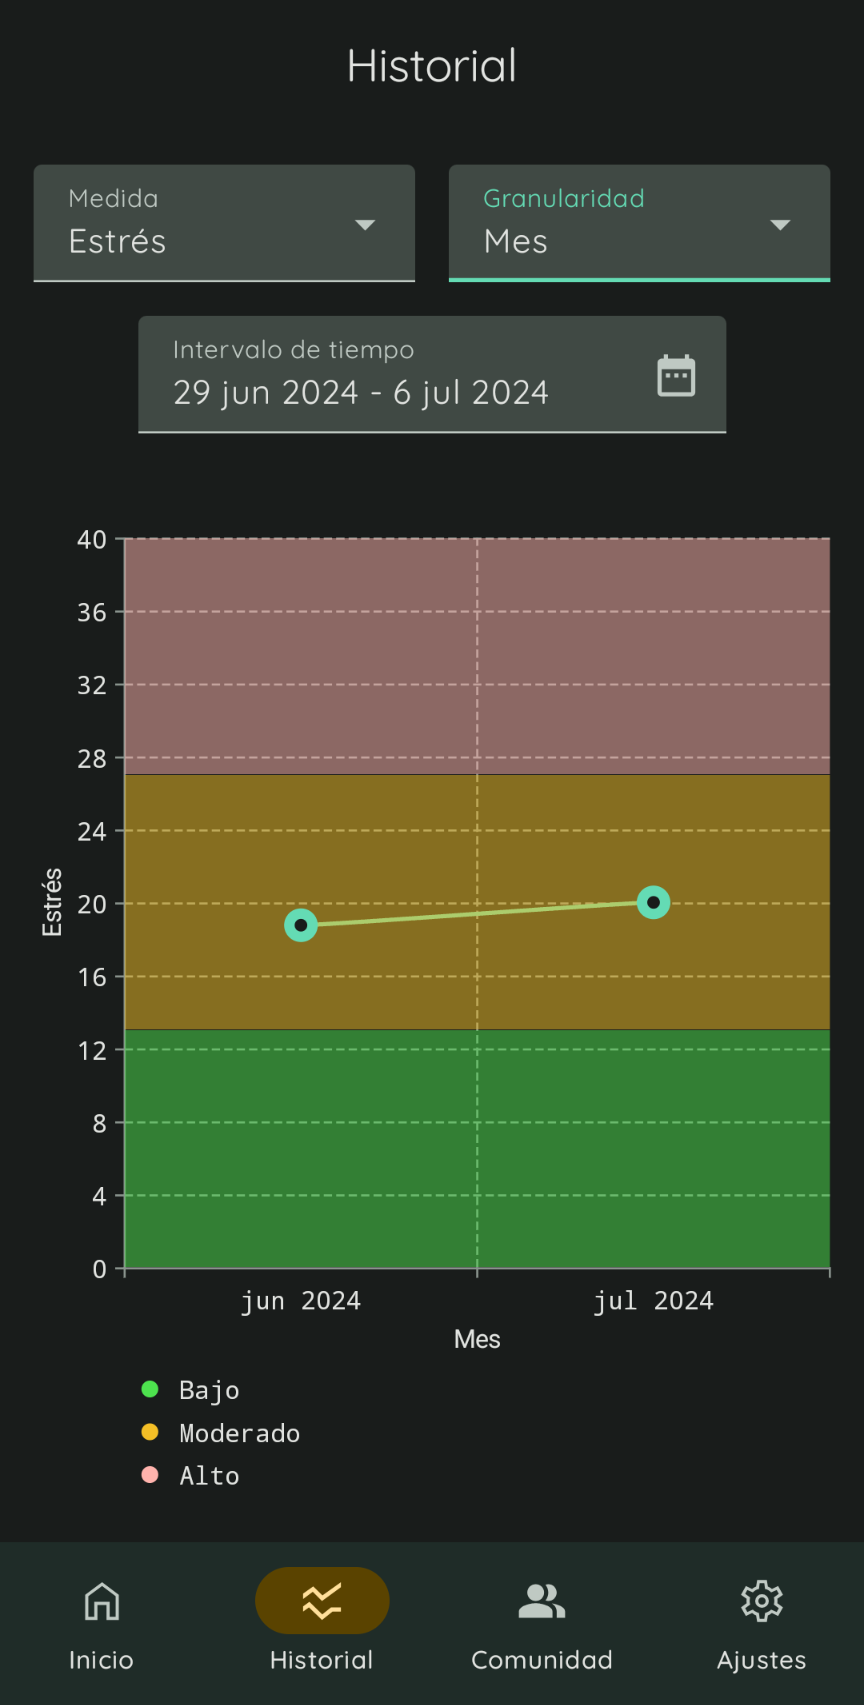
\includegraphics[width=1\linewidth]{figures/pruebas/visualizacion_estadistica/Grafica estres mes.png}
                \end{subfigure}
                \caption{Visualización estadística: flujo habitual}
                \label{figure:pruebas:visualizacion_estadistica}
            \end{figure}
            
            \clearpage  % Asegura que todas las figuras y tablas pendientes se impriman antes de continuar.
        \subsection*{Caso de prueba \textit{Uso de la aplicación en inglés}}
            Para visualizar la capacidad de la aplicación para mostrar textos en inglés se realizó un cambio en los ajustes y se reabrió la aplicación, como se puede ver en la Figura \ref{figure:pruebas:app_ingles}

            \begin{figure}[htbp]
                \centering
                \begin{subfigure}[c]{0.4\textwidth}
                    \centering
                    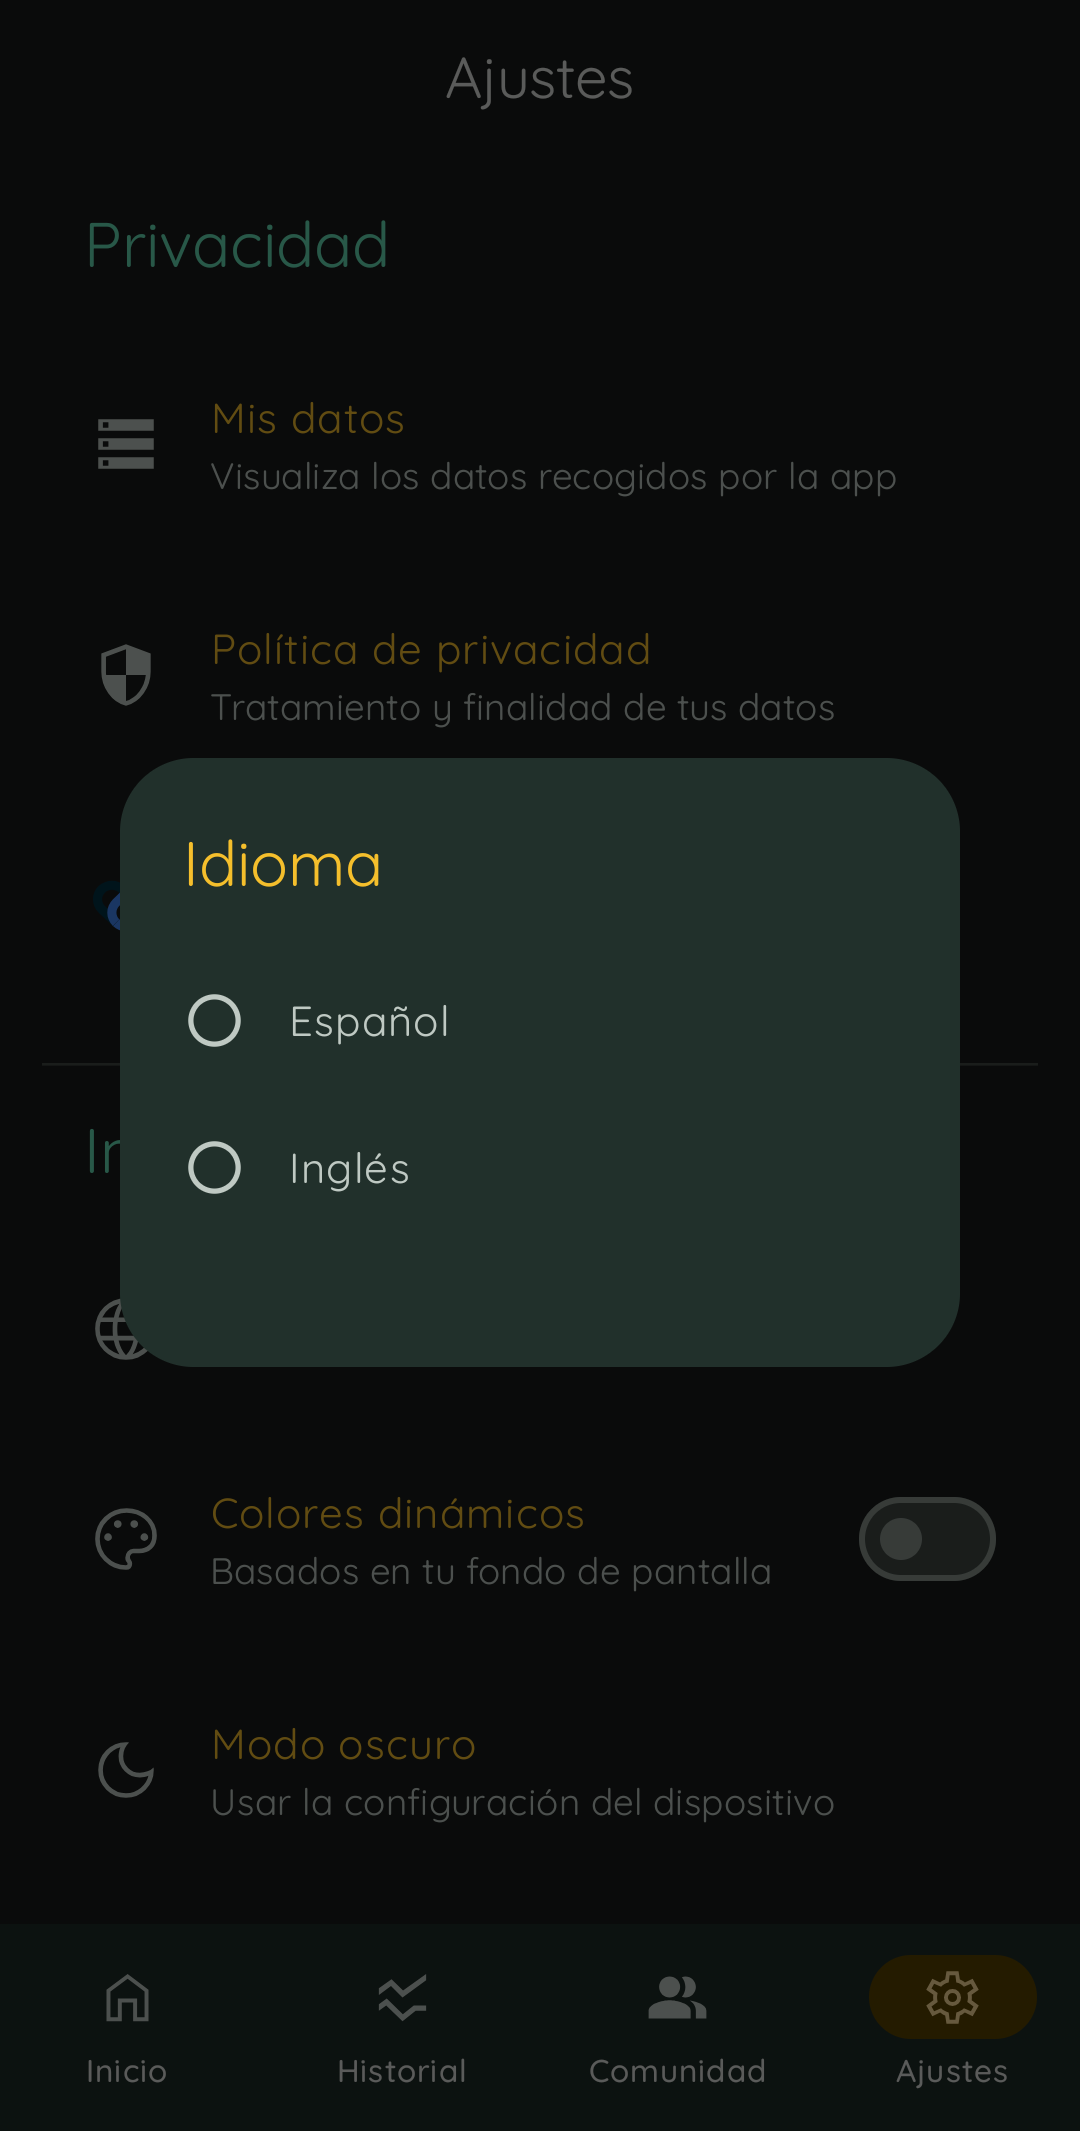
\includegraphics[width=1\textwidth]{figures/pruebas/ingles/Dialogo.png}
                \end{subfigure}
                \hspace{0.1\textwidth}
                \begin{subfigure}[c]{0.4\textwidth}
                    \centering
                    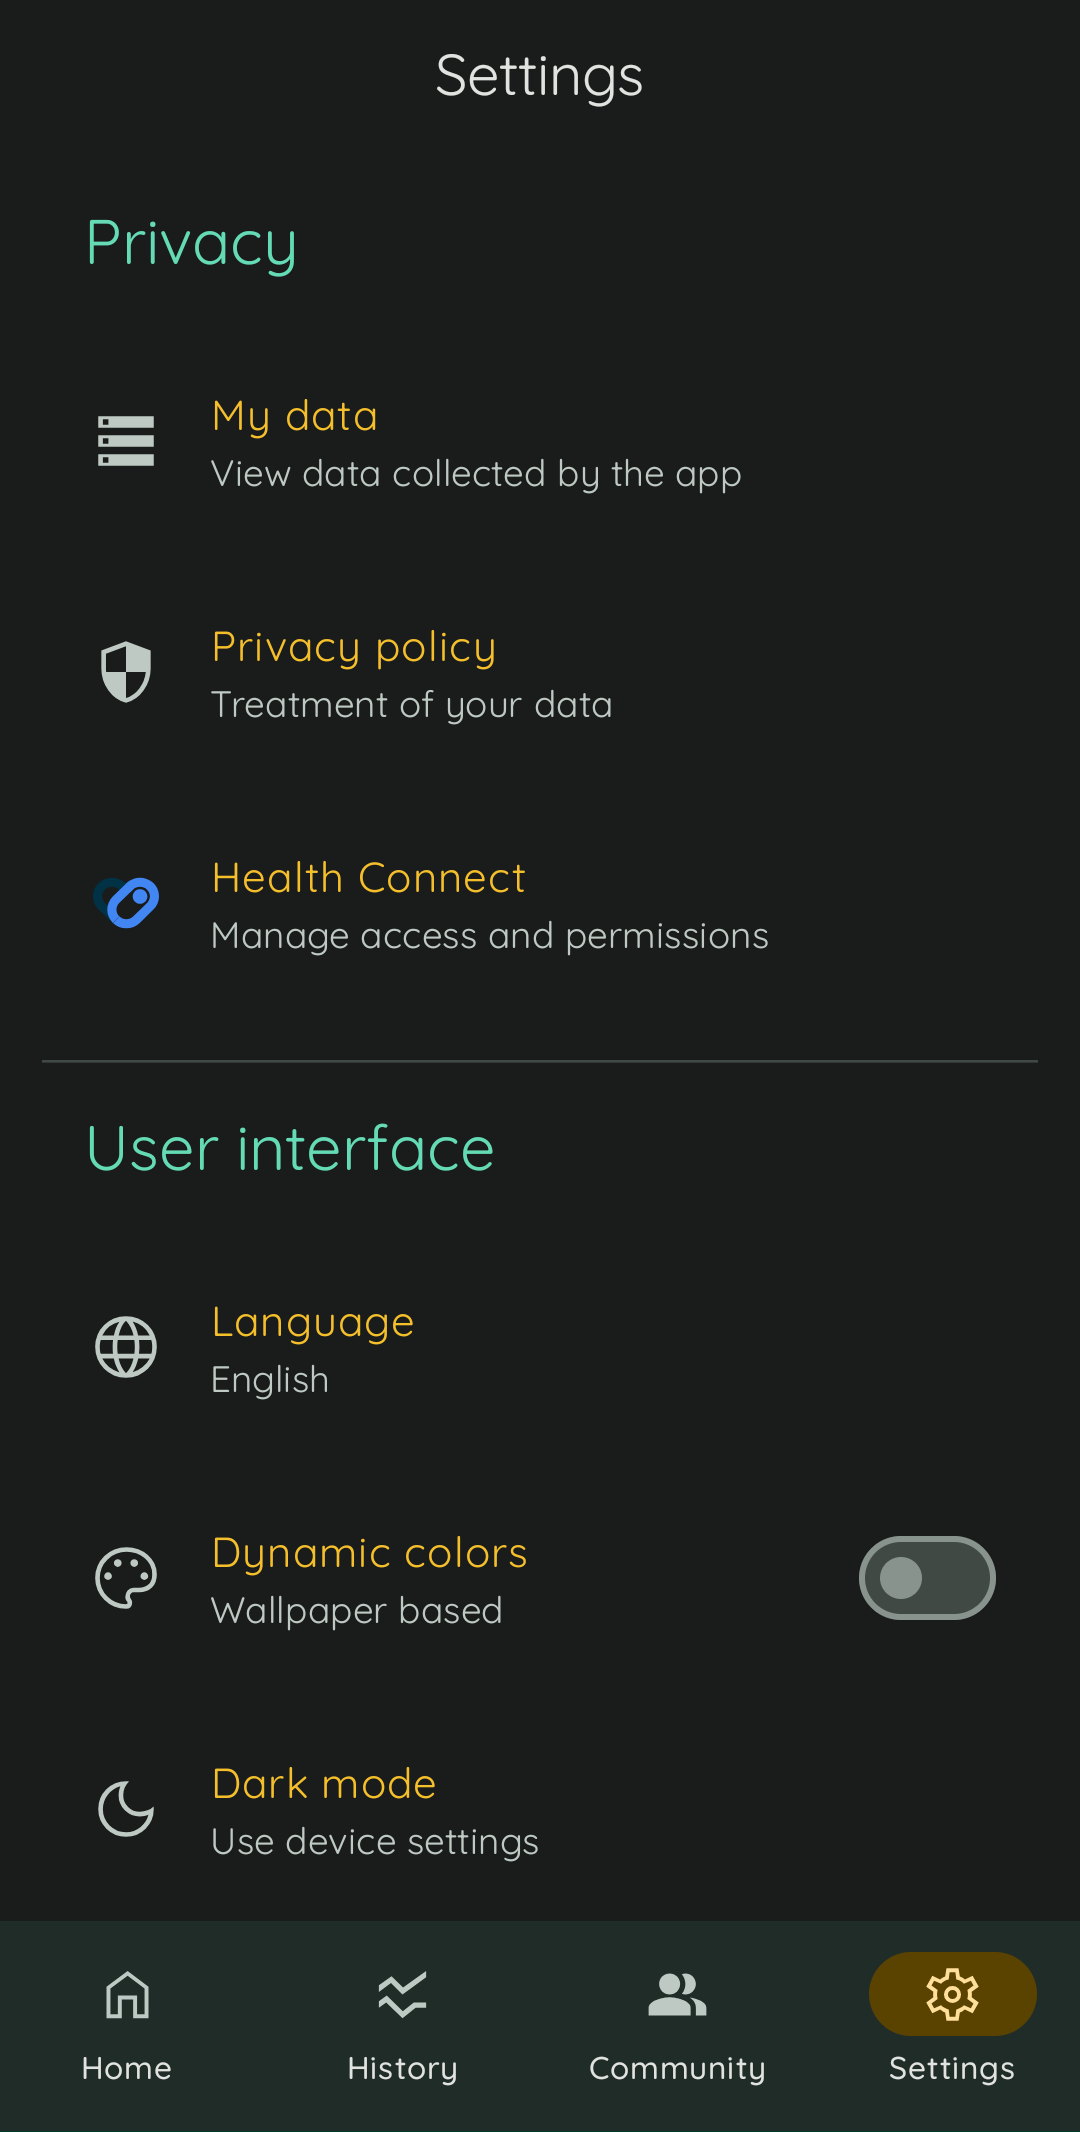
\includegraphics[width=1\linewidth]{figures/pruebas/ingles/Ingles.png}
                \end{subfigure}
                \caption{Evidencias del uso de la aplicación en inglés}
                \label{figure:pruebas:app_ingles}
            \end{figure}
            
        \subsection*{Caso de prueba \textit{Uso del modo claro de la aplicación}}
        
            Para visualizar la capacidad de la aplicación para utilizar el modo claro, se cambió el ajuste en el menú correspondiente, como se puede visualizar en la Figura \ref{figure:pruebas:modo_claro:ajuste}. 
            \begin{figure}[h]
                \centering
                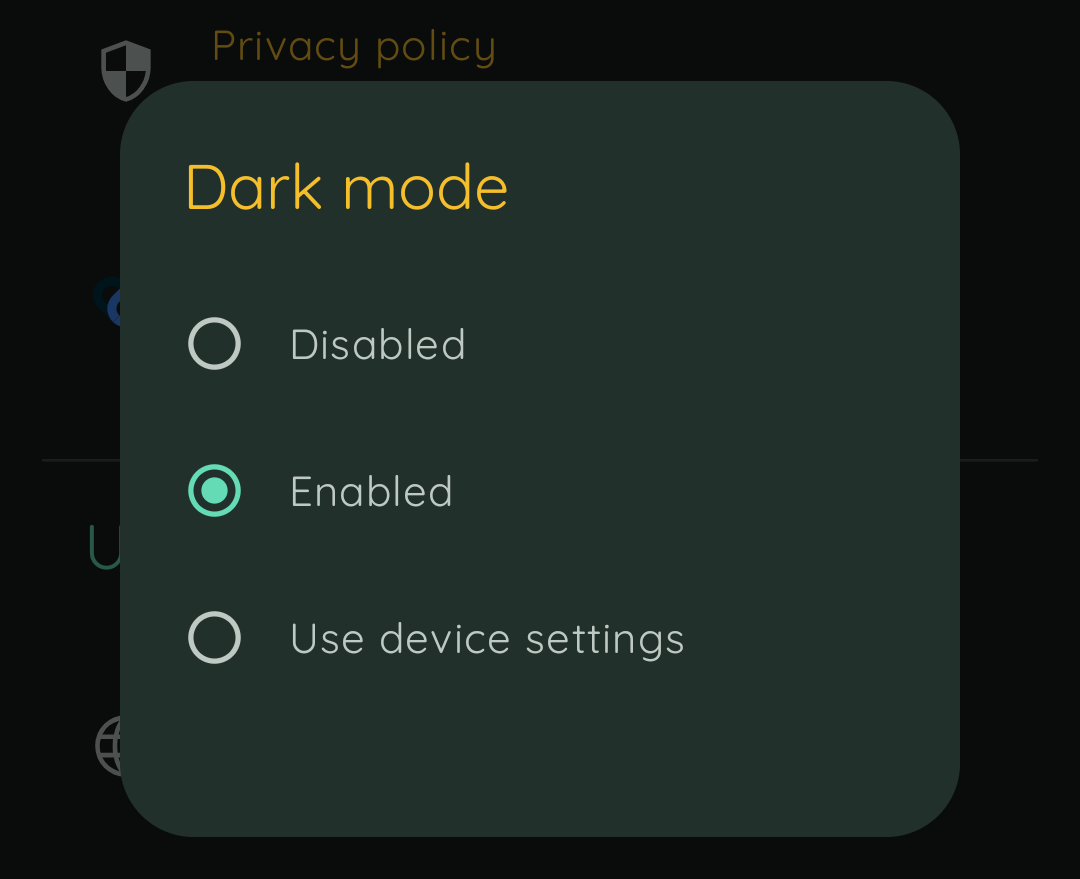
\includegraphics[width=0.4\textwidth]{figures/pruebas/modo_claro/Ajustes.png}
                \caption{Ajuste del cambio de modo de colores de la aplicación}
                \label{figure:pruebas:modo_claro:ajuste}
            \end{figure}

            Tras cambiar el ajuste, se reinició la aplicación, como se puede ver en la Figura  \ref{figure:pruebas:modo_claro}.
            
            \begin{figure}[htbp]
                \centering
                \begin{subfigure}[c]{0.4\textwidth}
                    \centering
                    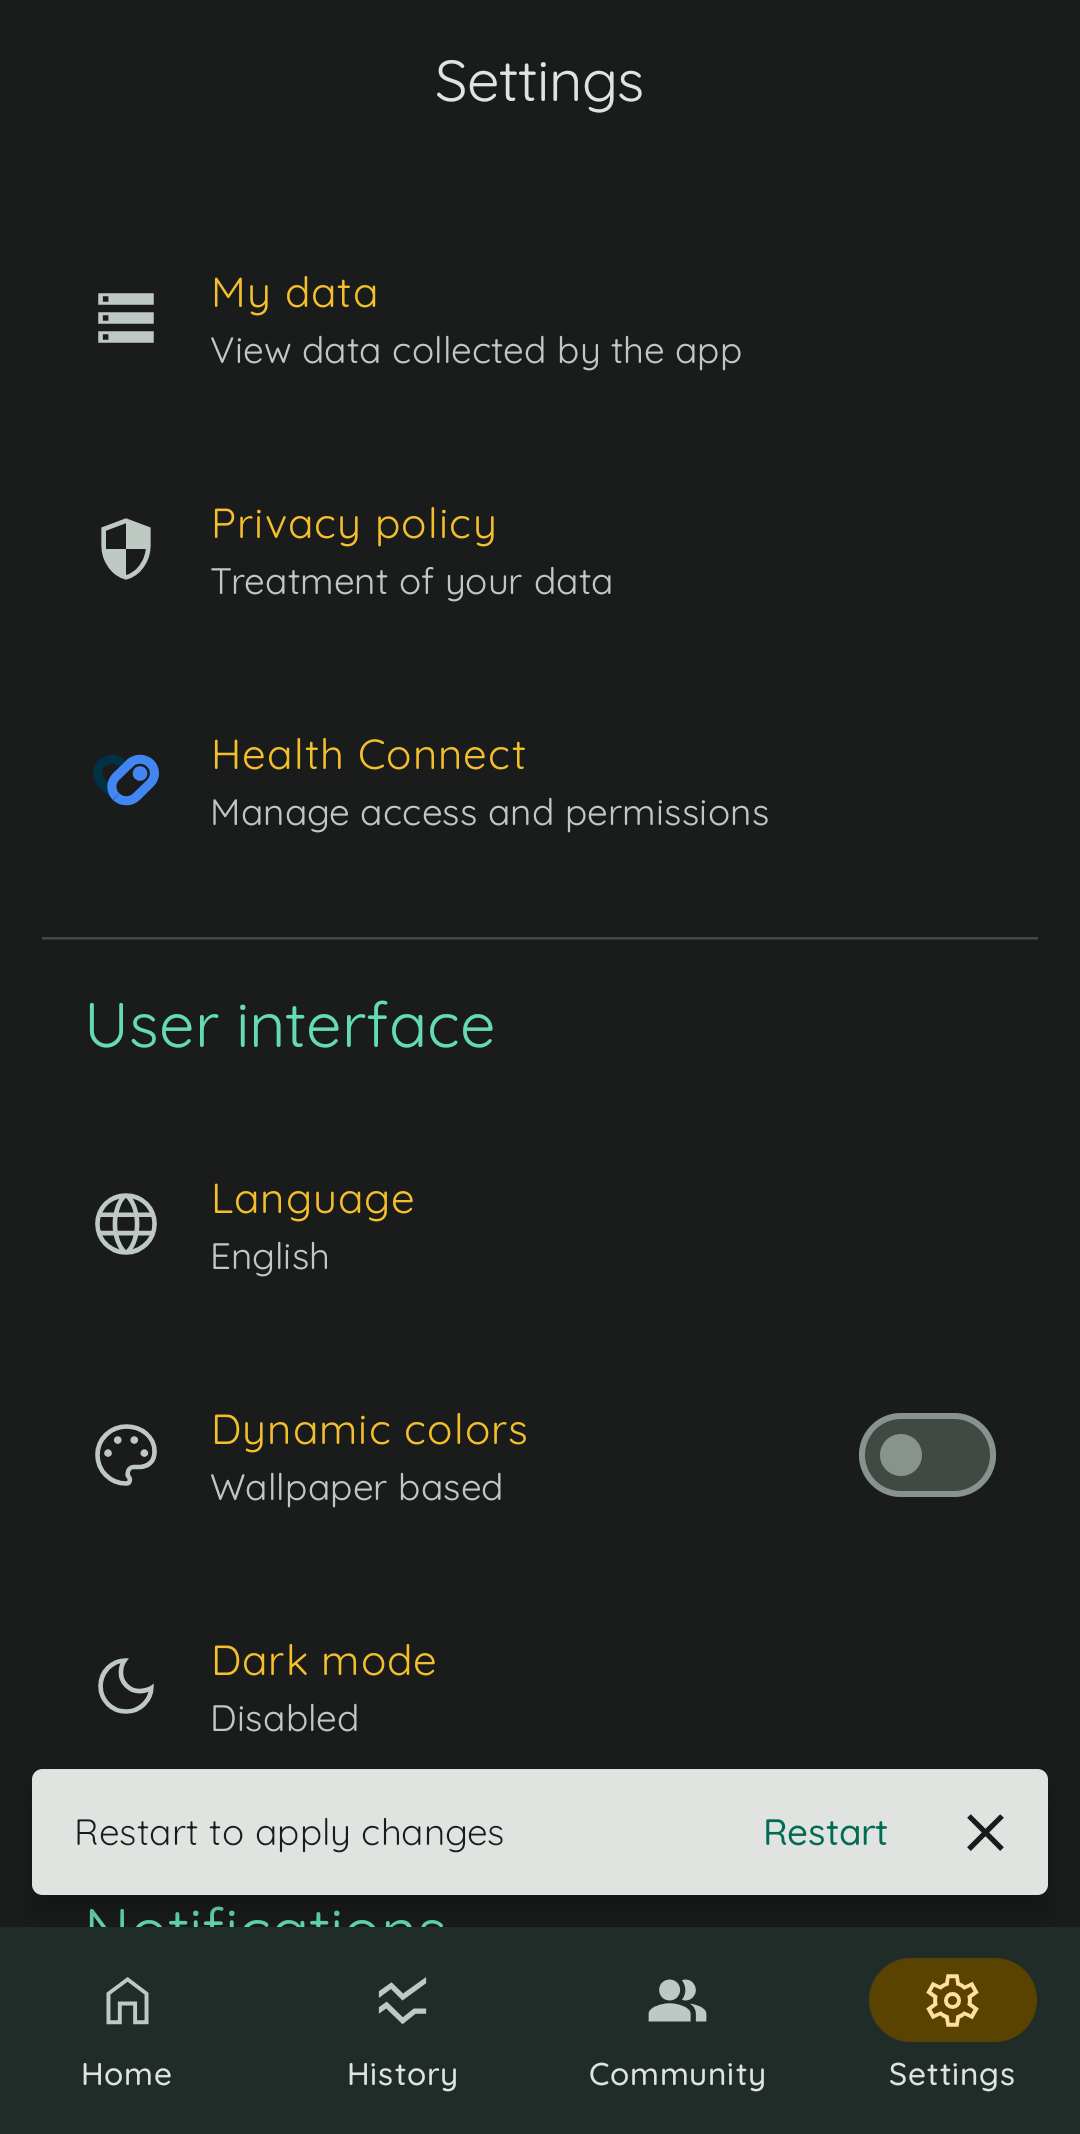
\includegraphics[width=1\textwidth]{figures/pruebas/modo_claro/Antes.png}
                \end{subfigure}
                \hspace{0.1\textwidth}
                \begin{subfigure}[c]{0.4\textwidth}
                    \centering
                    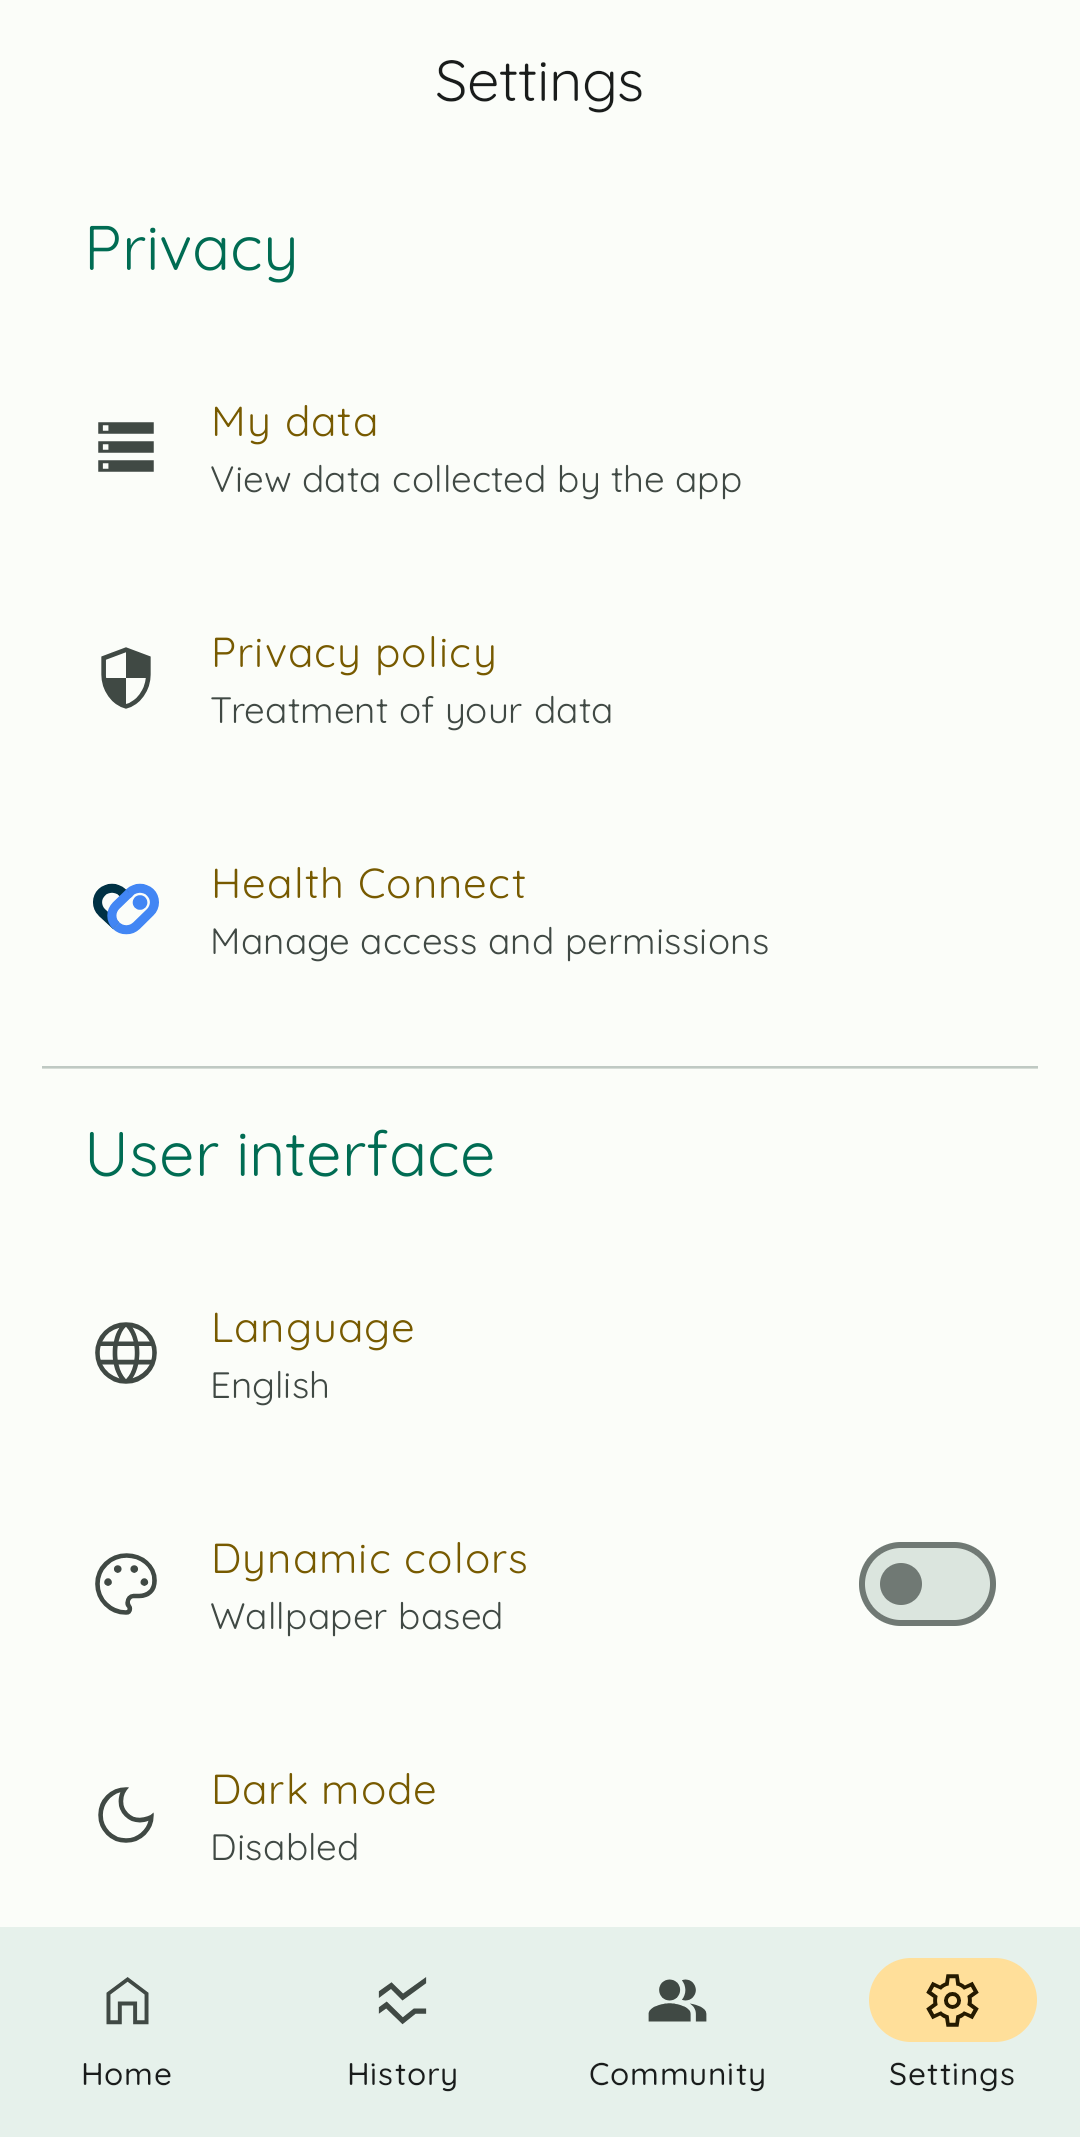
\includegraphics[width=1\linewidth]{figures/pruebas/modo_claro/Despues.png}
                \end{subfigure}
                \caption{Evidencias del uso del modo claro de la aplicación}
                \label{figure:pruebas:modo_claro}
            \end{figure}
            
            \clearpage  % Asegura que todas las figuras y tablas pendientes se impriman antes de continuar.
        \subsection*{Caso de prueba \textit{Uso del modo oscuro de la aplicación}}

            Análogamente al caso anterior, se cambió el ajuste en el menú correspondiente y se reinició la aplicación, como se refleja en la Figura \ref{figure:pruebas:modo_oscuro}.

            \begin{figure}[htbp]
                \centering
                \begin{subfigure}[c]{0.4\textwidth}
                    \centering
                    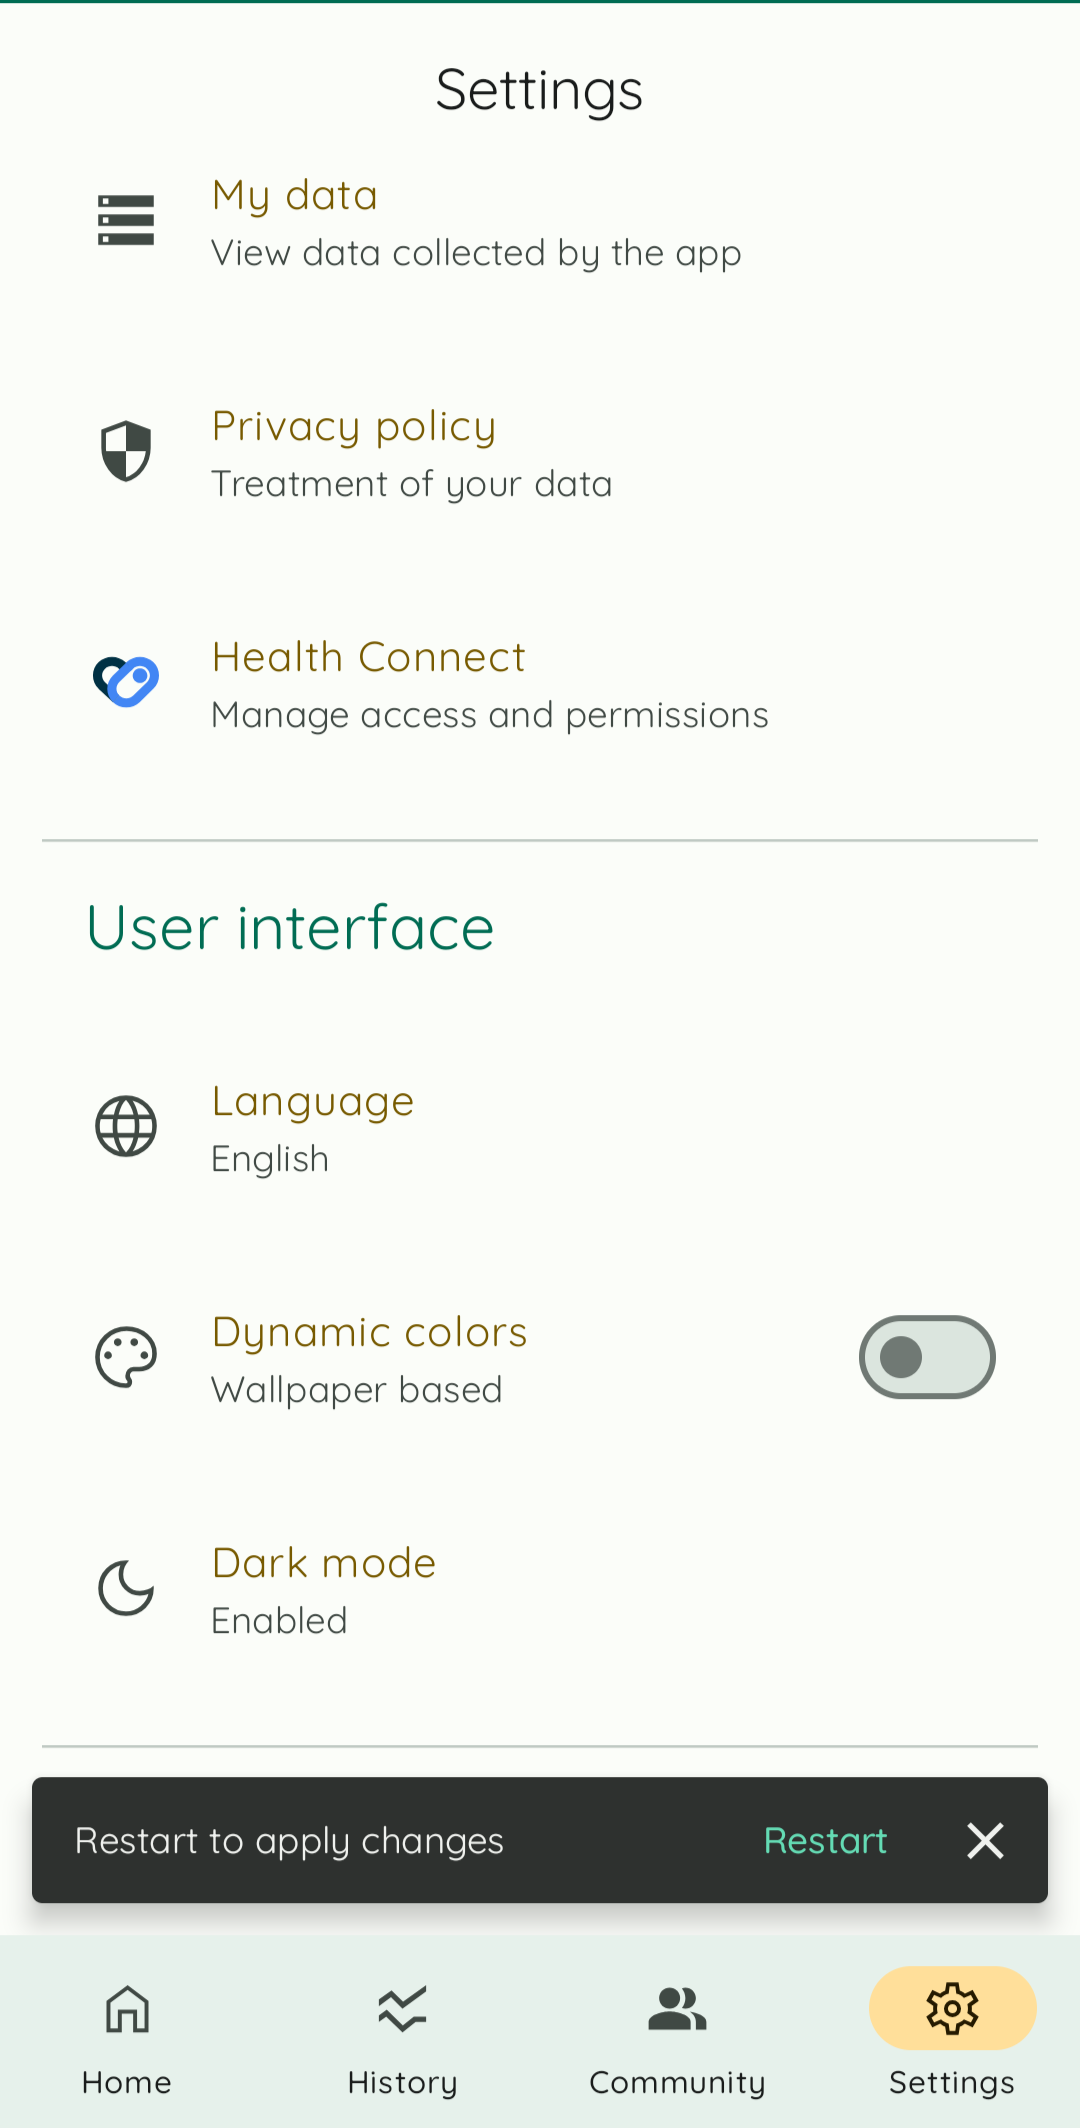
\includegraphics[width=1\textwidth]{figures/pruebas/modo_oscuro/Antes.png}
                \end{subfigure}
                \hspace{0.1\textwidth}
                \begin{subfigure}[c]{0.4\textwidth}
                    \centering
                    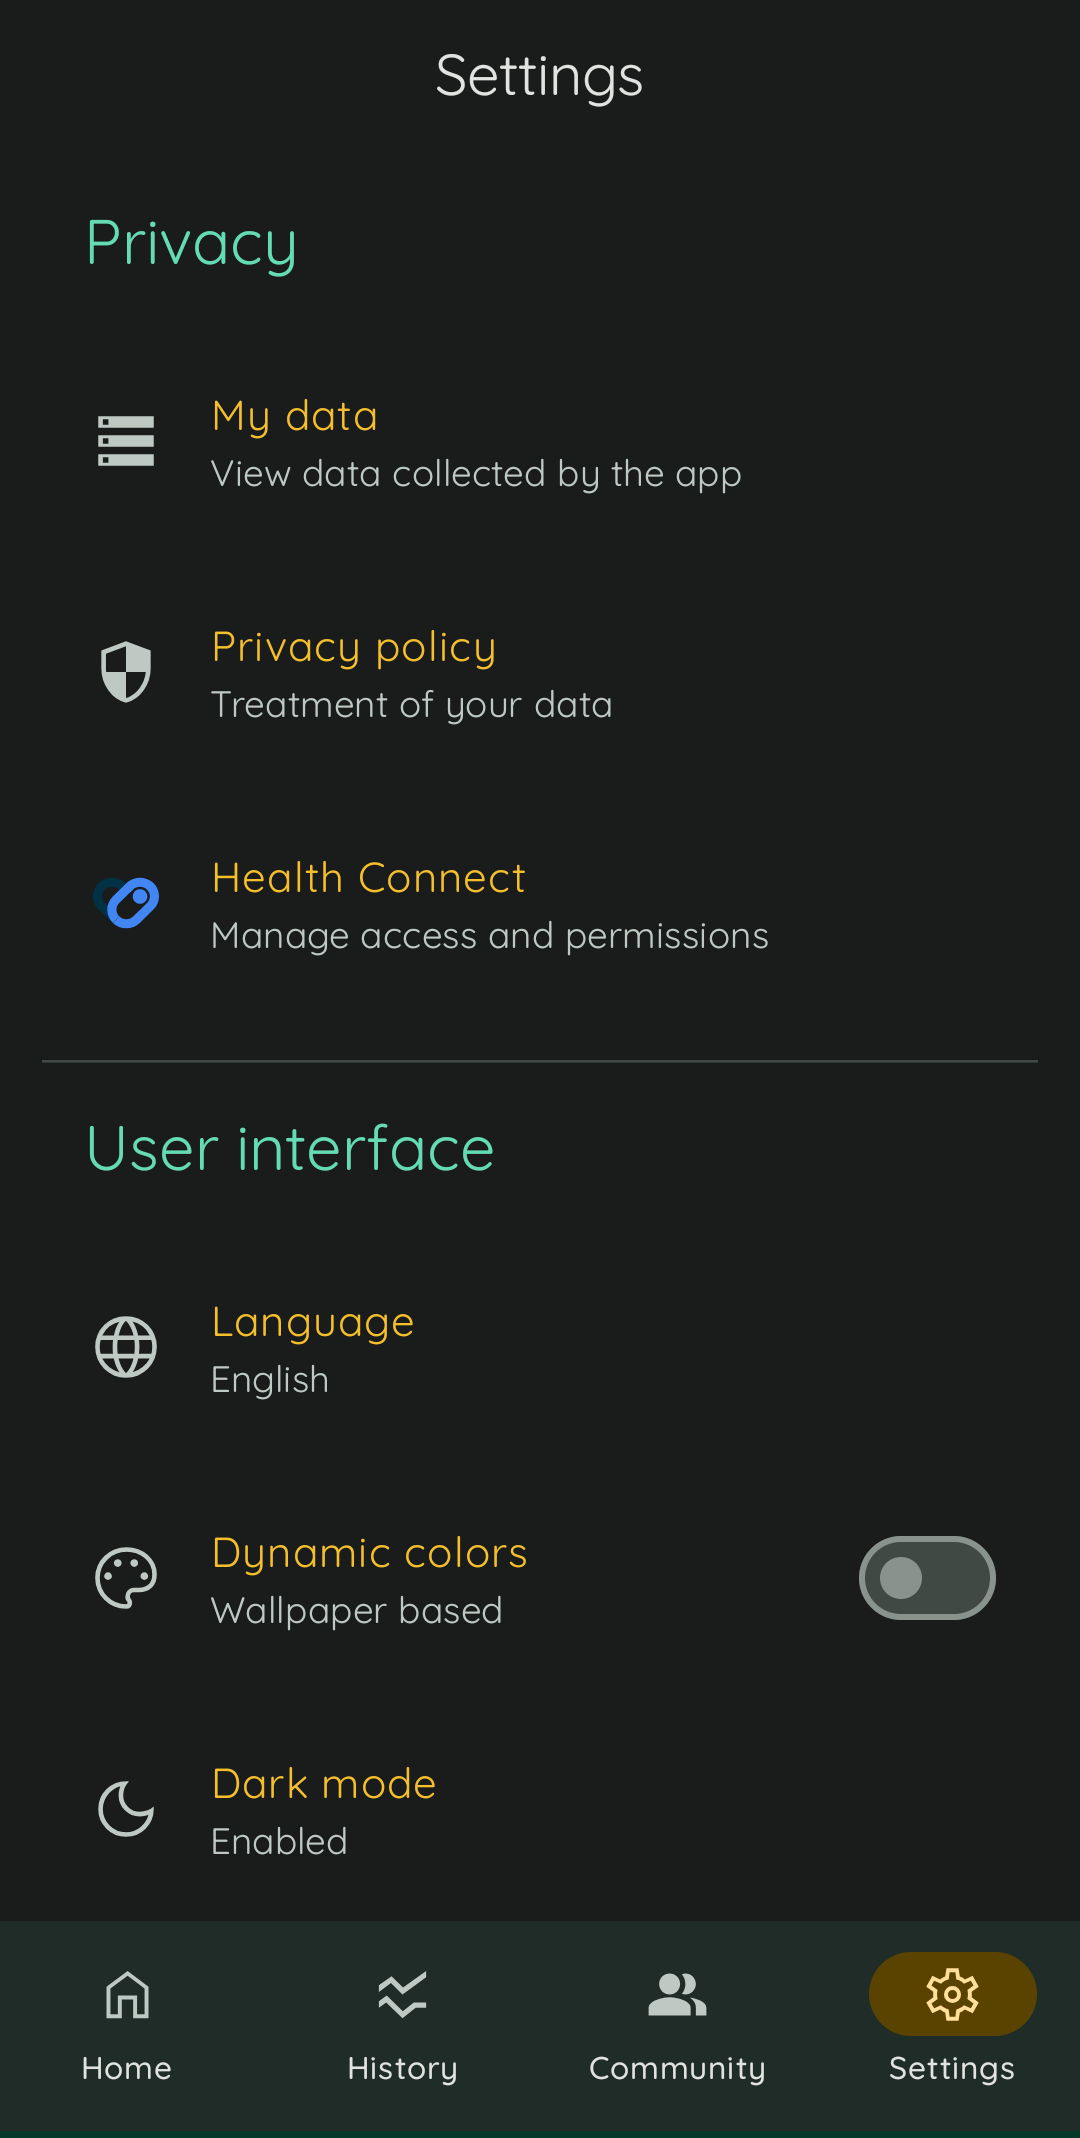
\includegraphics[width=1\linewidth]{figures/pruebas/modo_oscuro/Despues.png}
                \end{subfigure}
                \caption{Evidencias del uso del modo oscuro de la aplicación}
                \label{figure:pruebas:modo_oscuro}
            \end{figure}
            
        \subsection*{Caso de prueba \textit{Uso del esquema de colores dinámicos}}

            Para este último caso de prueba, se presenta en primer lugar el fondo del dispositivo en la Figura \ref{figure:pruebas:colores_dinamicos:inicio}, del cual Android extraerá la paleta de colores.

            \begin{figure}[h]
                \centering
                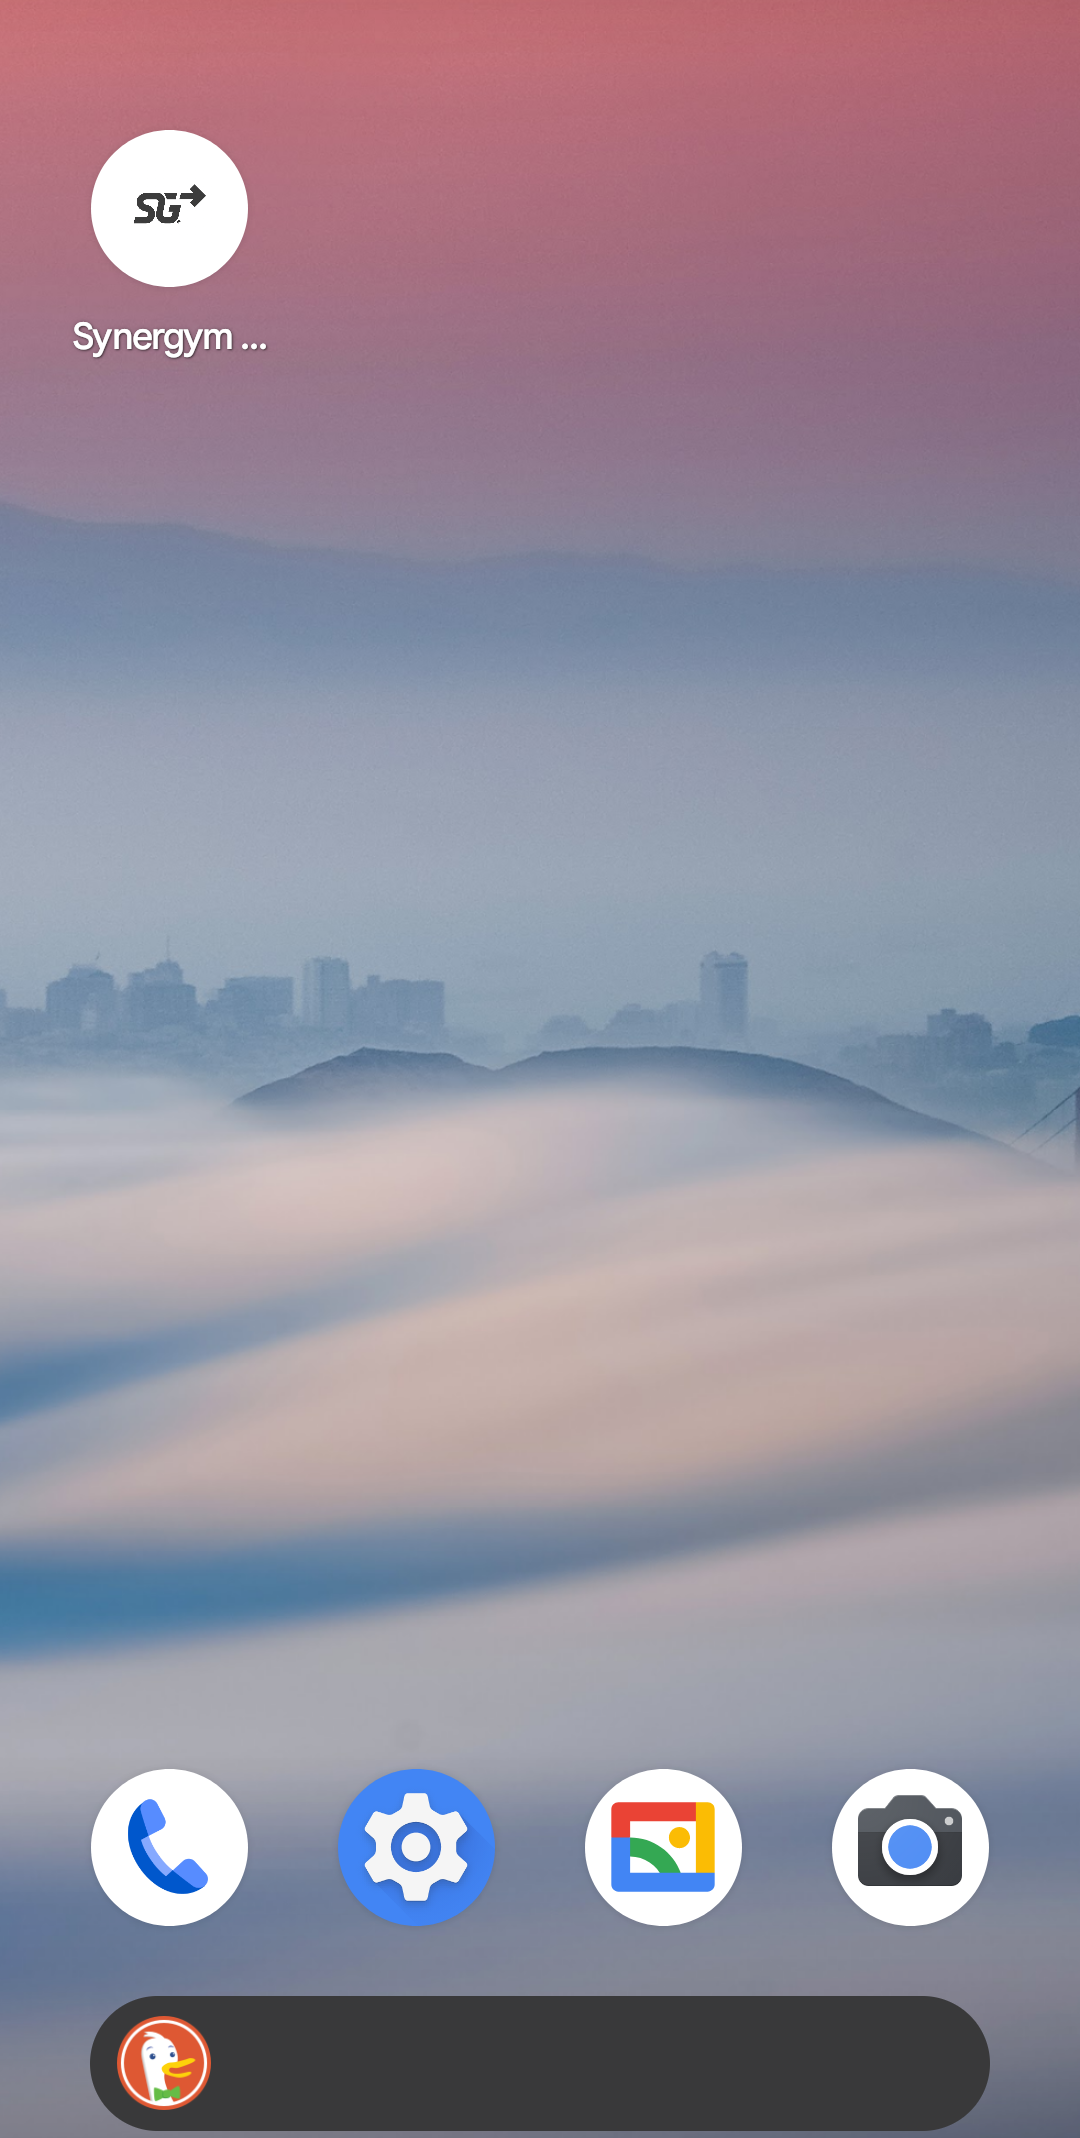
\includegraphics[width=0.25\textwidth]{figures/pruebas/colores_dinamicos/Inicio.png}
                \caption{Fondo de pantalla de ejemplo}
                \label{figure:pruebas:colores_dinamicos:inicio}
            \end{figure}

            Tras ello, nuevamente se cambió el ajuste en el menú correspondiente y se reinició la aplicación, como se indica en la Figura \ref{figure:pruebas:colores_dinamicos}.

            \begin{figure}[htbp]
                \centering
                \begin{subfigure}[c]{0.4\textwidth}
                    \centering
                    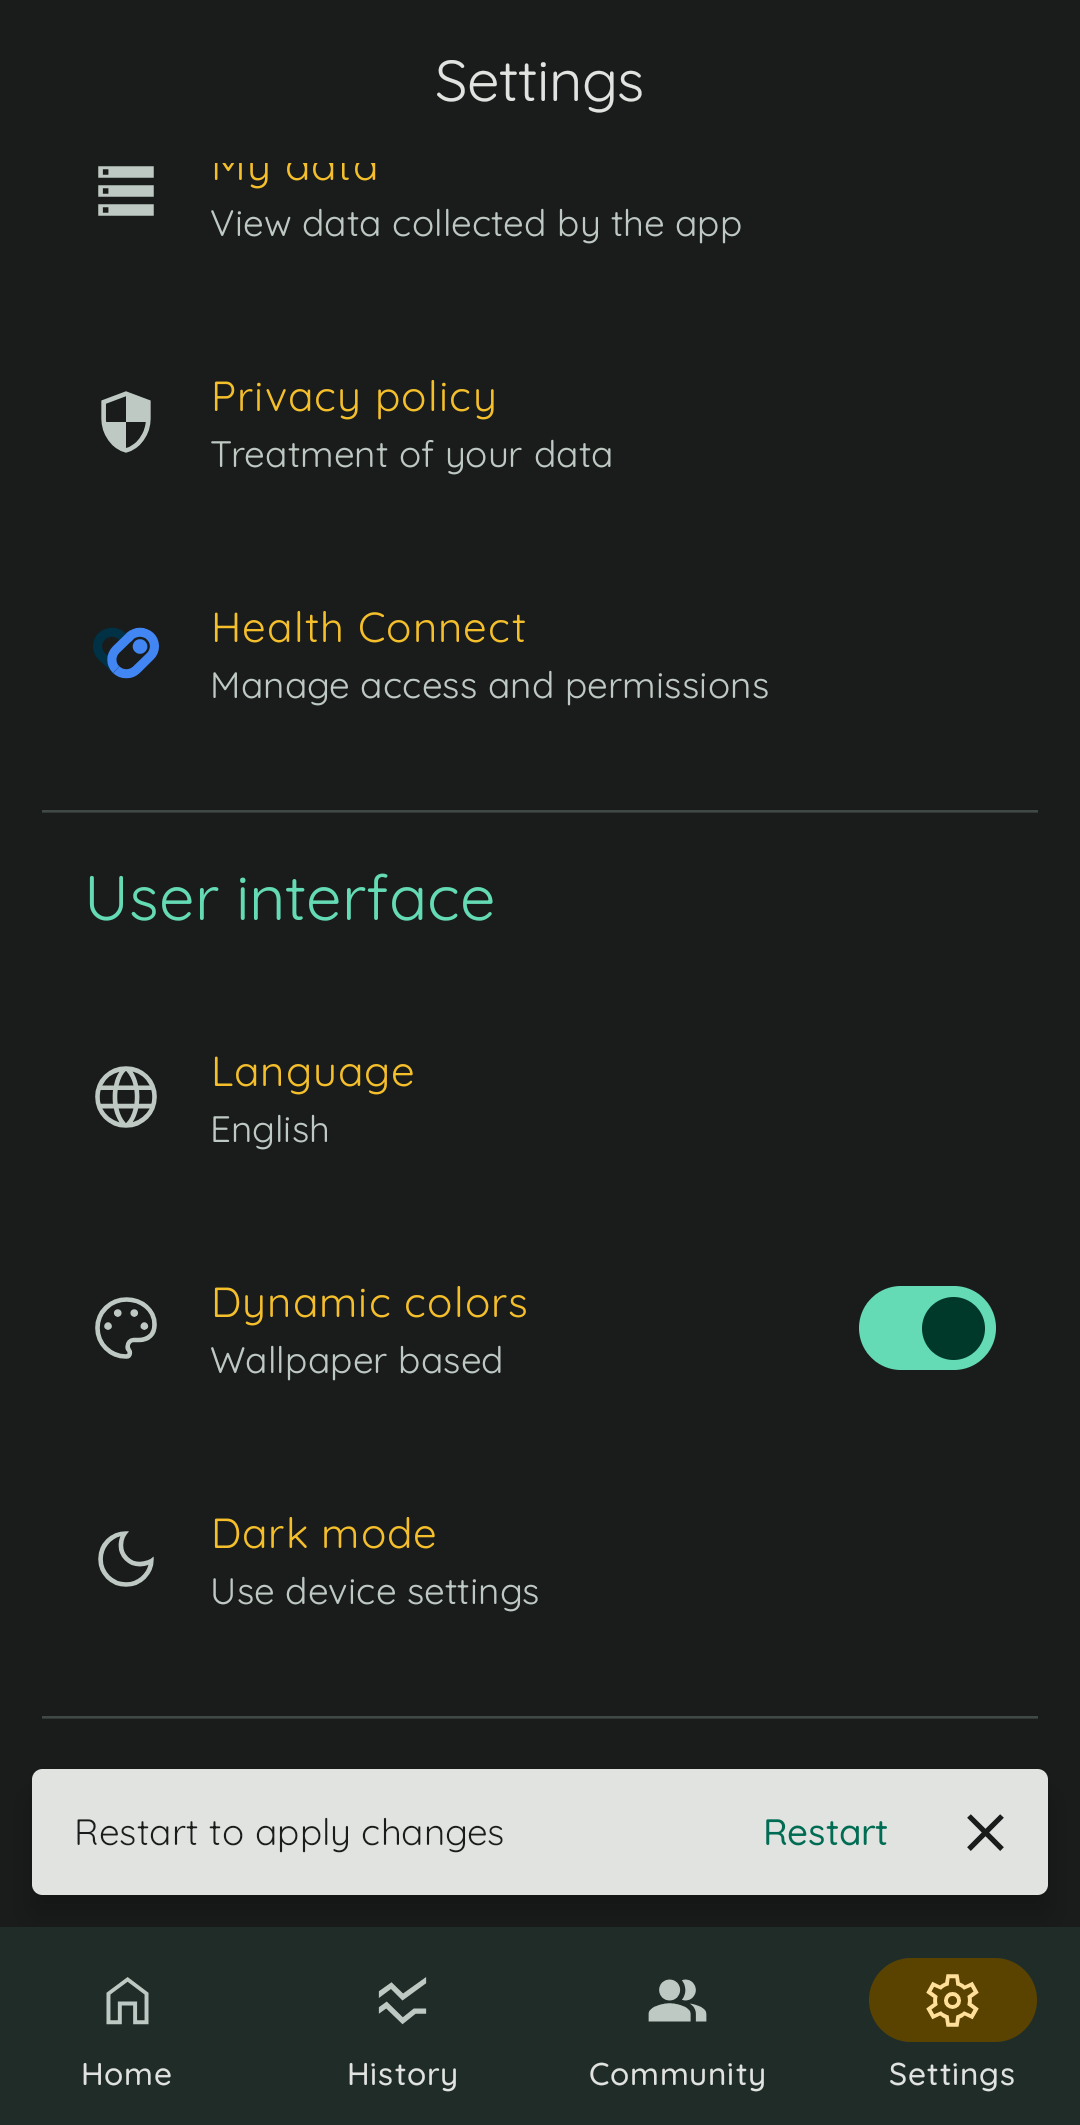
\includegraphics[width=1\textwidth]{figures/pruebas/colores_dinamicos/Antes.png}
                \end{subfigure}
                \hspace{0.1\textwidth}
                \begin{subfigure}[c]{0.4\textwidth}
                    \centering
                    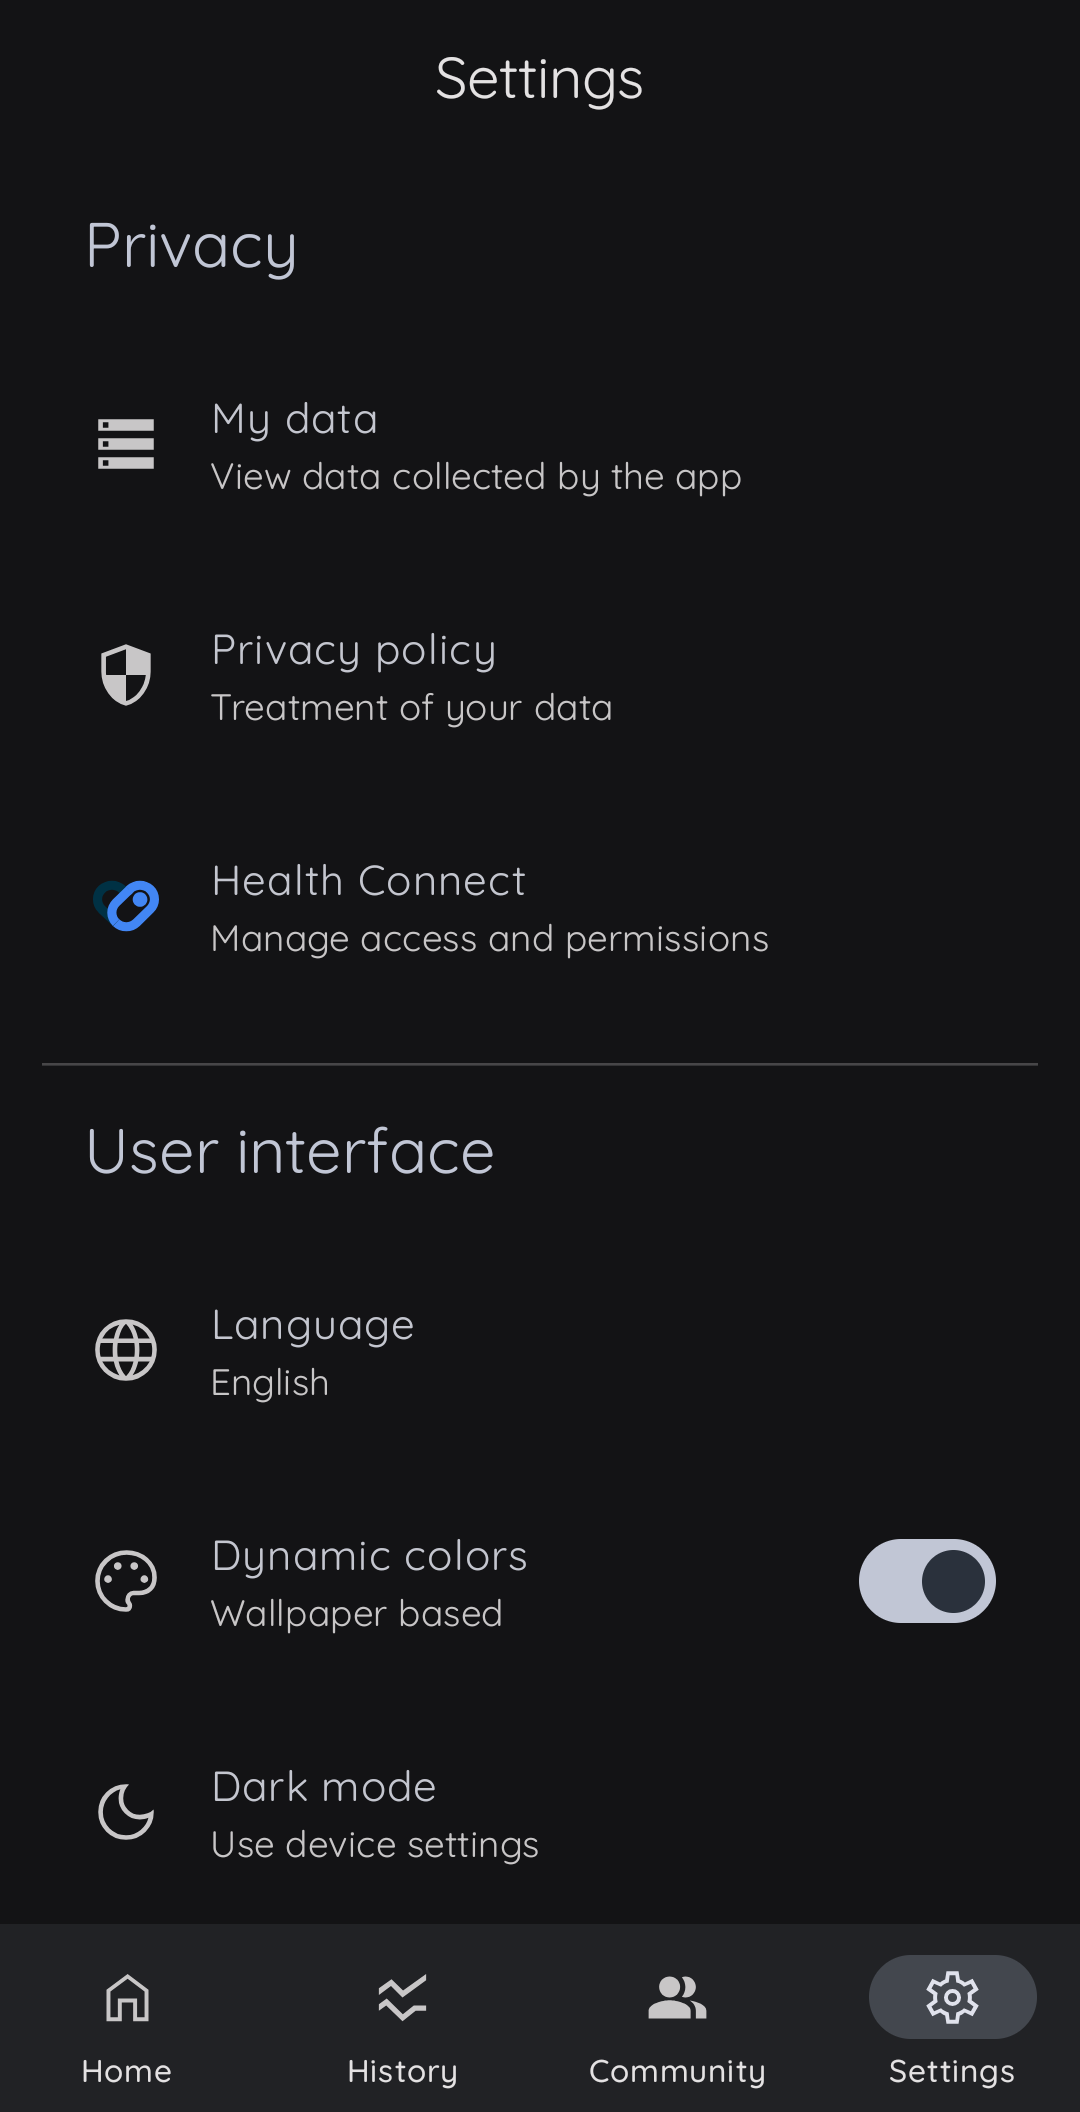
\includegraphics[width=1\linewidth]{figures/pruebas/colores_dinamicos/Despues.png}
                \end{subfigure}
                \caption{Evidencias del uso del esquema de colores dinámicos}
                \label{figure:pruebas:colores_dinamicos}
            \end{figure}
            
            \clearpage  % Asegura que todas las figuras y tablas pendientes se impriman antes de continuar.

    \section{Pruebas del sistema}
        En esta sección se van a describir las pruebas realizadas a las funcionalidades que involucran varios componentes.
        
        \subsection*{Caso de prueba \textit{Sincronización de los datos del dispositivo wearable}}

            Para el envío de datos entre la aplicación y el servidor de actividad física se recogen en las Figuras \ref{figure:pruebas:sincronizacion_wearable:movil} y \ref{figure:pruebas:sincronizacion_wearable:servidor} las trazas recogidas del intercambio de información.

            \begin{figure}[h]
                \centering
                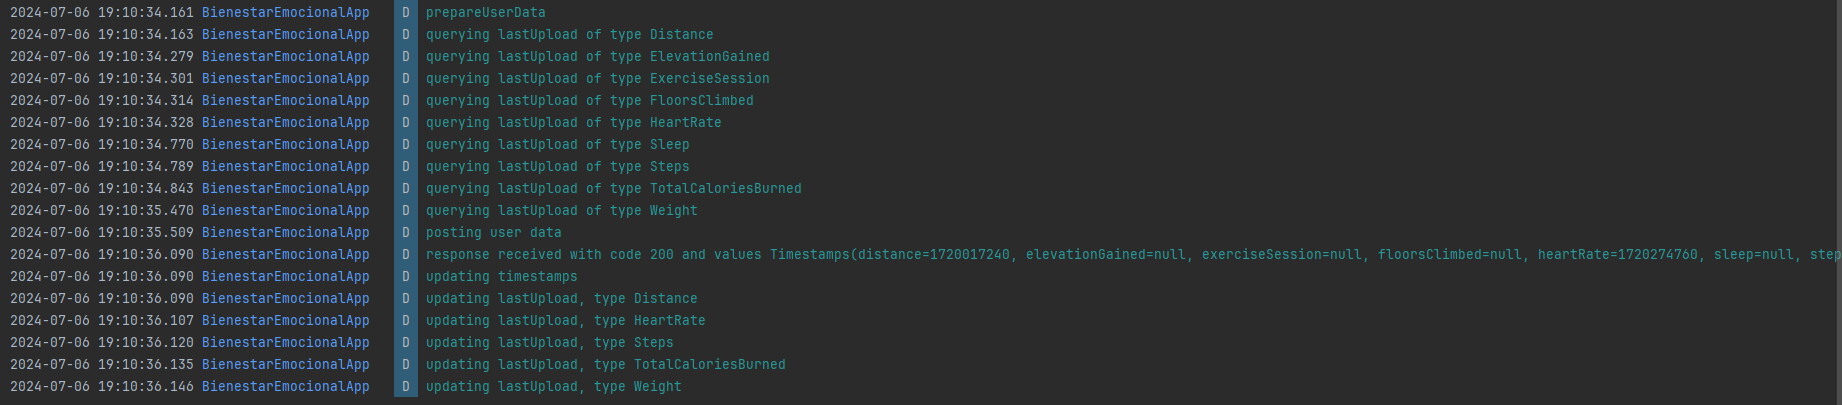
\includegraphics[width=1\textwidth]{figures/pruebas/sincro_wearable/Traza movil.png}
                \caption{Traza móvil de la sincronización de datos del wearable}
                \label{figure:pruebas:sincronizacion_wearable:movil}
            \end{figure}

            \begin{figure}[h]
                \centering
                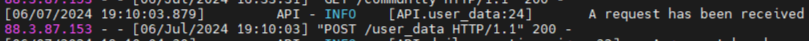
\includegraphics[width=1\textwidth]{figures/pruebas/sincro_wearable/Traza servidor.png}
                \caption{Traza servidor de la sincronización de datos del wearable}
                \label{figure:pruebas:sincronizacion_wearable:servidor}
            \end{figure}

    
        \subsection*{Caso de prueba \textit{Sincronización de los datos de seguimiento}}

            Para el envío de datos entre la aplicación y el servidor de los datos de seguimiento (cuestionarios) se recogen en las Figuras \ref{figure:pruebas:sincronizacion_cuestionarios:movil} y \ref{figure:pruebas:sincronizacion_cuestionarios:servidor} las trazas recogidas del intercambio de información.

            \begin{figure}[h]
                \centering
                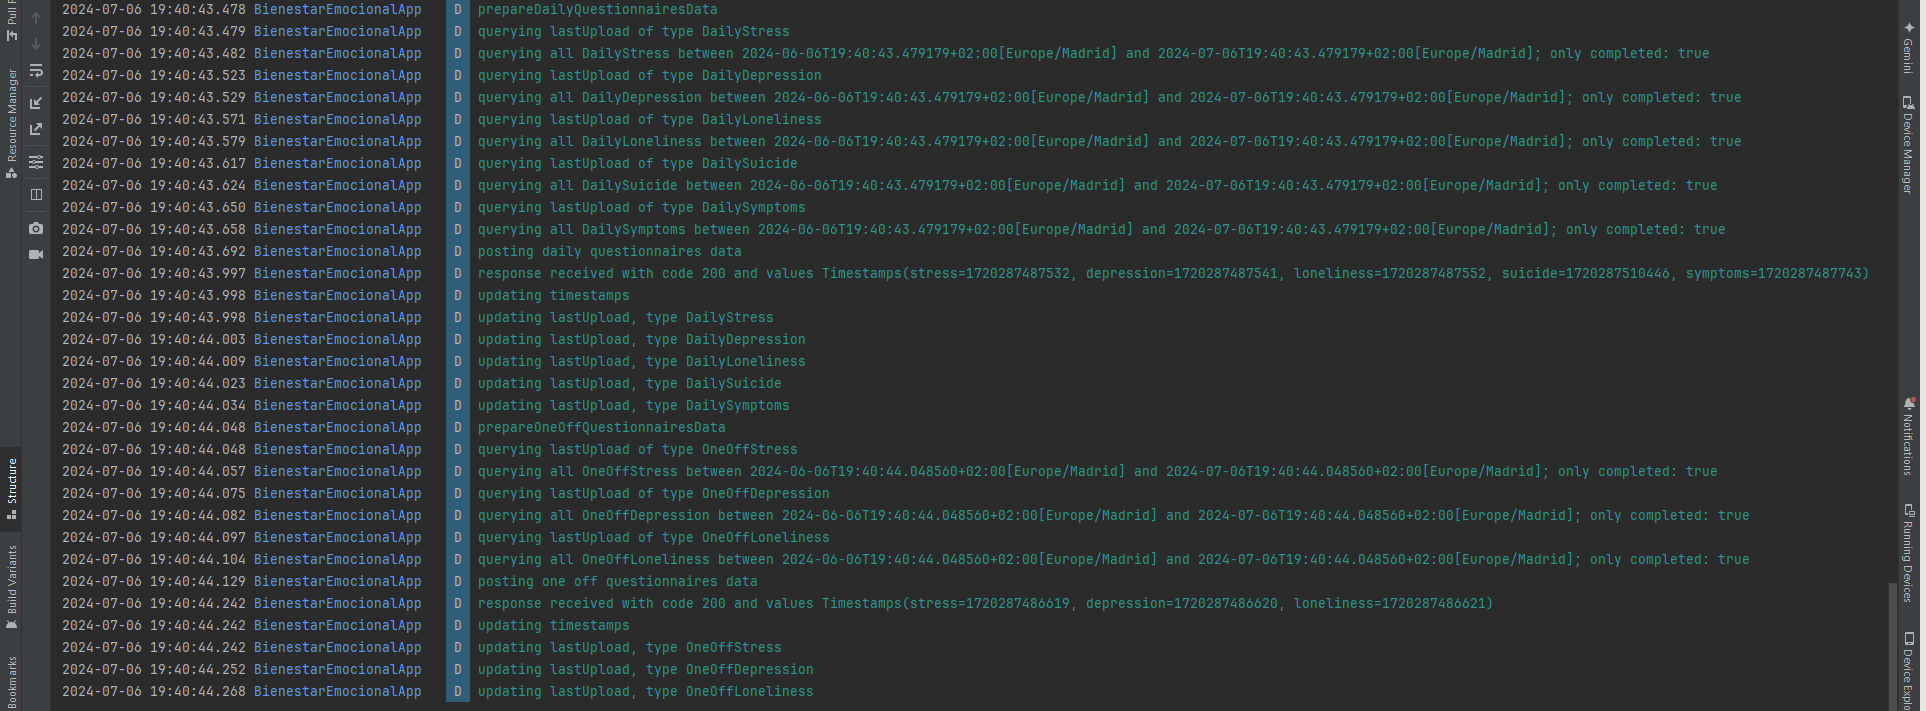
\includegraphics[width=1\textwidth]{figures/pruebas/sincro_cuestionarios/Trazas movil.png}
                \caption{Traza móvil de la sincronización de datos de seguimiento}
                \label{figure:pruebas:sincronizacion_cuestionarios:movil}
            \end{figure}

            \begin{figure}[h]
                \centering
                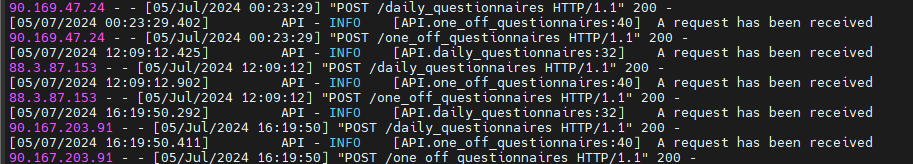
\includegraphics[width=1\textwidth]{figures/pruebas/sincro_cuestionarios/Trazas servidor.png}
                \caption{Traza servidor  de la sincronización de datos de seguimiento}
                \label{figure:pruebas:sincronizacion_cuestionarios:servidor}
            \end{figure}

            \clearpage  % Asegura que todas las figuras y tablas pendientes se impriman antes de continuar.
            
        \subsection*{Caso de prueba \textit{Visualización conjunta}}

            En la Figura \ref{figure:pruebas:visualizacion_conjunta} se muestra cómo la aplicación muestra la visualización conjunta, en los casos de depresión y soledad respectivamente.

            \begin{figure}[htbp]
                \centering
                \begin{subfigure}[c]{0.4\textwidth}
                    \centering
                    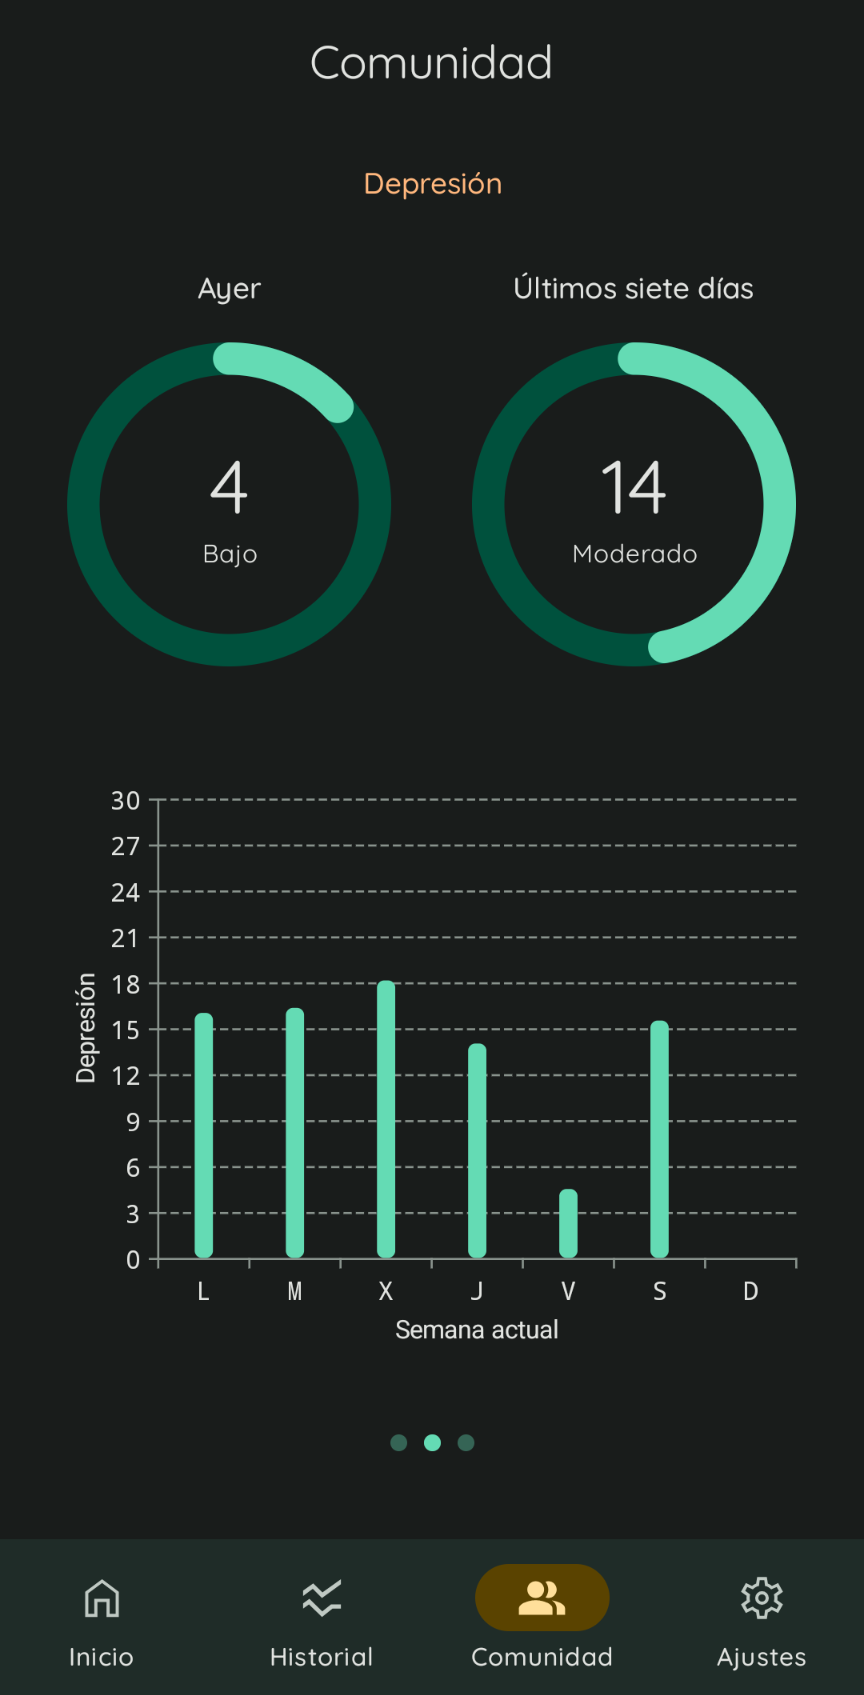
\includegraphics[width=1\textwidth]{figures/pruebas/comunidad/Comunidad depresion.png}
                \end{subfigure}
                \hspace{0.1\textwidth}
                \begin{subfigure}[c]{0.4\textwidth}
                    \centering
                    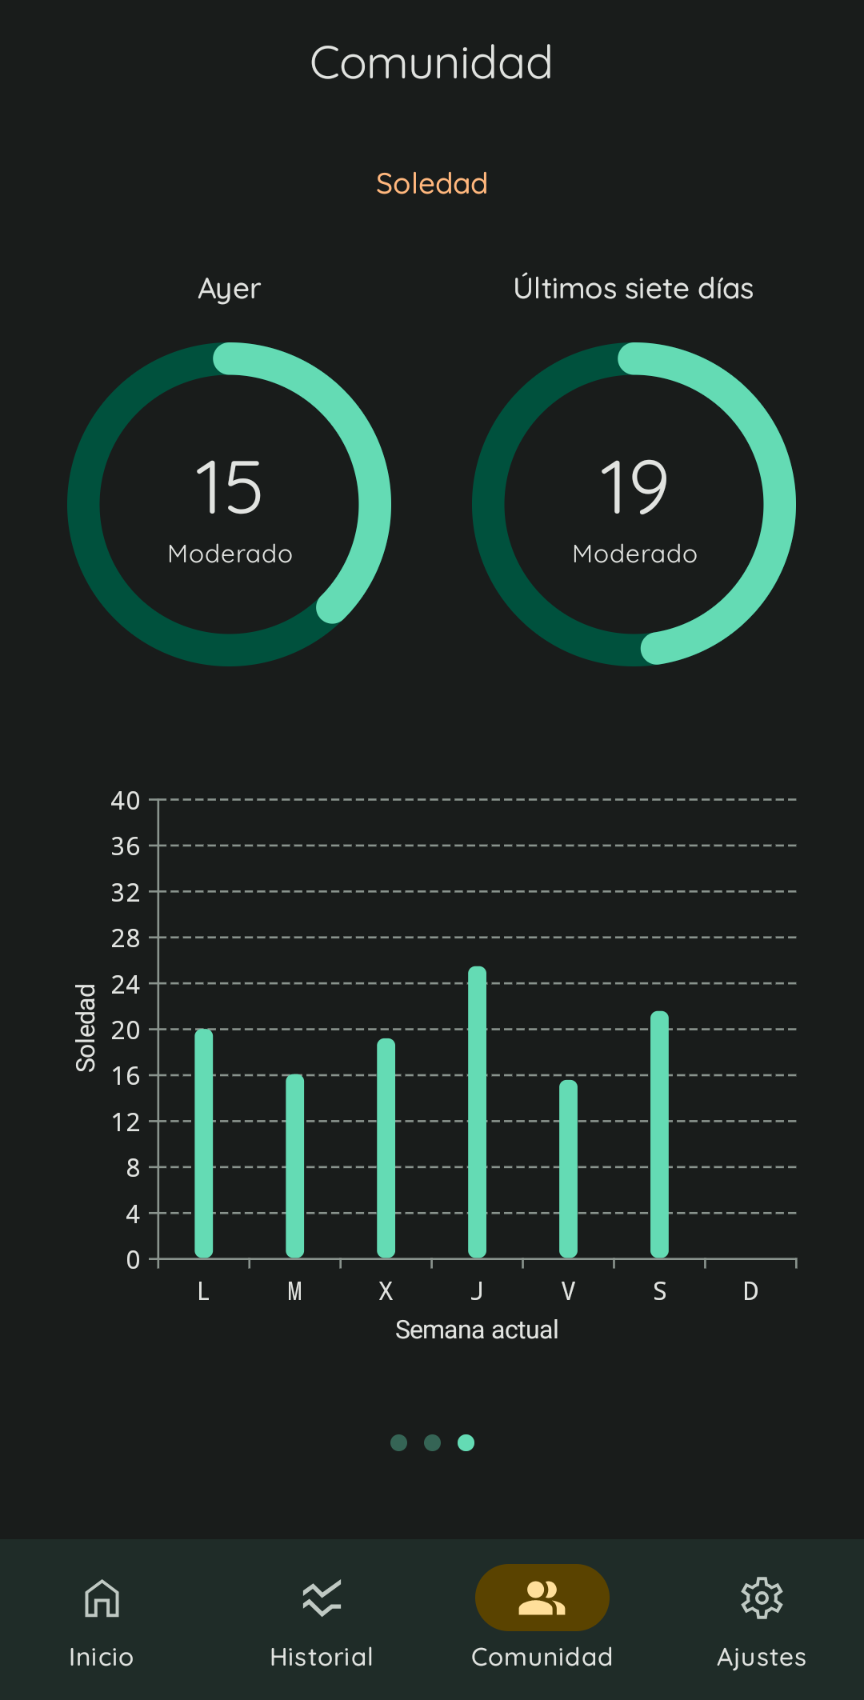
\includegraphics[width=1\linewidth]{figures/pruebas/comunidad/Comunidad soledad.png}
                \end{subfigure}
                \caption{Visualización conjunta}
                \label{figure:pruebas:visualizacion_conjunta}
            \end{figure}

            Por último, como en los casos anteriores, se muestran en las Figuras \ref{figure:pruebas:comunidad:movil} y \ref{figure:pruebas:comunidad:servidor} las trazas recogidas del intercambio de información.
            
            \begin{figure}[h]
                \centering
                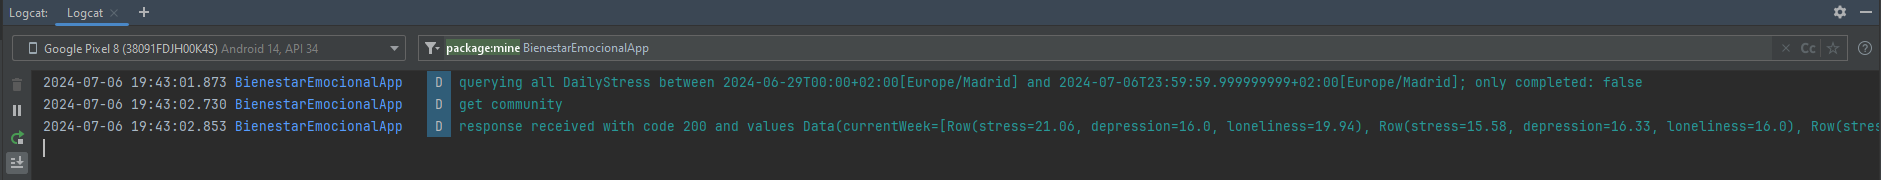
\includegraphics[width=1\textwidth]{figures/pruebas/comunidad/Traza movil.png}
                \caption{Traza móvil de la visualización conjunta}
                \label{figure:pruebas:comunidad:movil}
            \end{figure}

            \begin{figure}[h]
                \centering
                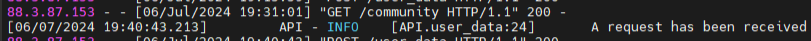
\includegraphics[width=1\textwidth]{figures/pruebas/comunidad/Traza servidor.png}
                \caption{Traza servidor de la visualización conjunta}
                \label{figure:pruebas:comunidad:servidor}
            \end{figure}